\documentclass[11pt]{article}
% =======================================================================
%   Shared style for CS 300 notes.
%   Usage: place `% =======================================================================
%   Shared style for CS 300 notes.
%   Usage: place `% =======================================================================
%   Shared style for CS 300 notes.
%   Usage: place `\input{../../notes-style.tex}` right after \documentclass
%   in each chapter's lectures.tex and notes.tex.
% =======================================================================

% ---- Layout -----------------------------------------------------------
\usepackage[margin=1in]{geometry}
\usepackage{parskip}        % space between paragraphs, no indent
\usepackage{microtype}      % subtle kerning/spacing improvements

% ---- Colors (muted palette, easy on light-sensitive eyes) -------------
\usepackage{xcolor}
\definecolor{pagebg}       {HTML}{FAF6F0}  % warm cream background
\definecolor{bodyfg}       {HTML}{3D3A36}  % warm dark gray body text
\definecolor{heading}      {HTML}{3D6A6B}  % muted teal
\definecolor{subheading}   {HTML}{5B7A9C}  % dusty blue
\definecolor{accent}       {HTML}{8A6B4A}  % warm tan
\definecolor{linkcol}      {HTML}{5B7A9C}  % same as subheading
\definecolor{mutedtext}    {HTML}{6B6560}  % secondary / caption text
\definecolor{rulecol}      {HTML}{C8BFB0}  % separator / rule

% Callout box palette
\definecolor{defnFrame}    {HTML}{9DB89B}  \definecolor{defnBack}    {HTML}{EEF2E8}
\definecolor{ideaFrame}    {HTML}{9FB4CD}  \definecolor{ideaBack}    {HTML}{E8EEF5}
\definecolor{warnFrame}    {HTML}{CFAE87}  \definecolor{warnBack}    {HTML}{F5EDDF}
\definecolor{noteFrame}    {HTML}{BFA6AE}  \definecolor{noteBack}    {HTML}{F2E8EE}
\definecolor{exFrame}      {HTML}{9FBDBD}  \definecolor{exBack}      {HTML}{E8F0F0}
\definecolor{codeBack}     {HTML}{F3EDE2}
\definecolor{codeBorder}   {HTML}{D4CBBA}
\definecolor{codeKeyword}  {HTML}{6B4F7A}
\definecolor{codeString}   {HTML}{8A6B4A}
\definecolor{codeComment}  {HTML}{8A857F}

% ---- Page background + base text color --------------------------------
\usepackage{pagecolor}
\pagecolor{pagebg}
\color{bodyfg}

% ---- Fonts ------------------------------------------------------------
\usepackage[T1]{fontenc}
\IfFileExists{libertine.sty}{%
    \usepackage{libertine}      % warm, readable serif
    \usepackage[scaled=0.95]{inconsolata}  % softer monospace
}{}

% ---- Hyperref ---------------------------------------------------------
\usepackage{hyperref}
\hypersetup{
    colorlinks=true,
    linkcolor=linkcol,
    urlcolor=linkcol,
    citecolor=linkcol,
    pdfborder={0 0 0},
}

% ---- Section styling --------------------------------------------------
\usepackage[explicit]{titlesec}
\titleformat{\section}
    {\color{heading}\Large\bfseries}
    {\color{heading}\thesection\hspace{0.6em}}{0pt}{#1}
\titleformat{\subsection}
    {\color{subheading}\large\bfseries}
    {\color{subheading}\thesubsection\hspace{0.5em}}{0pt}{#1}
\titleformat{\subsubsection}
    {\color{accent}\normalsize\bfseries}
    {\color{accent}\thesubsubsection\hspace{0.5em}}{0pt}{#1}
\titleformat{\paragraph}[runin]
    {\color{accent}\bfseries}{}{0pt}{#1.}

\titlespacing*{\section}{0pt}{1.6em}{0.6em}
\titlespacing*{\subsection}{0pt}{1.2em}{0.4em}

% ---- Enumerate / itemize spacing --------------------------------------
\usepackage{enumitem}
\setlist[itemize]{leftmargin=1.4em, itemsep=2pt, topsep=4pt}
\setlist[enumerate]{leftmargin=1.6em, itemsep=2pt, topsep=4pt}

% ---- Code listings ----------------------------------------------------
\usepackage{listings}
\lstdefinestyle{notescode}{
    backgroundcolor=\color{codeBack},
    basicstyle=\ttfamily\small\color{bodyfg},
    keywordstyle=\color{codeKeyword}\bfseries,
    stringstyle=\color{codeString},
    commentstyle=\color{codeComment}\itshape,
    frame=single,
    framesep=6pt,
    rulecolor=\color{codeBorder},
    showstringspaces=false,
    breaklines=true,
    xleftmargin=10pt,
    xrightmargin=10pt,
    aboveskip=8pt,
    belowskip=8pt,
}
\lstset{style=notescode}

% ---- Callout boxes (tcolorbox) ----------------------------------------
\usepackage[most]{tcolorbox}

\newtcolorbox{defnbox}[1][]{
    enhanced, breakable,
    colback=defnBack, colframe=defnFrame, coltitle=bodyfg,
    title={\bfseries Definition \textemdash\ #1},
    fonttitle=\bfseries,
    boxrule=0.5pt, arc=2pt, left=8pt, right=8pt, top=6pt, bottom=6pt,
    attach boxed title to top left={xshift=10pt, yshift=-6pt},
    boxed title style={colback=defnFrame, colframe=defnFrame, arc=2pt},
    before skip=8pt, after skip=8pt,
}
\newtcolorbox{ideabox}[1][]{
    enhanced, breakable,
    colback=ideaBack, colframe=ideaFrame, coltitle=bodyfg,
    title={\bfseries Key idea #1},
    boxrule=0.5pt, arc=2pt, left=8pt, right=8pt, top=6pt, bottom=6pt,
    attach boxed title to top left={xshift=10pt, yshift=-6pt},
    boxed title style={colback=ideaFrame, colframe=ideaFrame, arc=2pt},
    before skip=8pt, after skip=8pt,
}
\newtcolorbox{warnbox}[1][]{
    enhanced, breakable,
    colback=warnBack, colframe=warnFrame, coltitle=bodyfg,
    title={\bfseries Gotcha #1},
    boxrule=0.5pt, arc=2pt, left=8pt, right=8pt, top=6pt, bottom=6pt,
    attach boxed title to top left={xshift=10pt, yshift=-6pt},
    boxed title style={colback=warnFrame, colframe=warnFrame, arc=2pt},
    before skip=8pt, after skip=8pt,
}
\newtcolorbox{notebox}[1][]{
    enhanced, breakable,
    colback=noteBack, colframe=noteFrame, coltitle=bodyfg,
    title={\bfseries Aside #1},
    boxrule=0.5pt, arc=2pt, left=8pt, right=8pt, top=6pt, bottom=6pt,
    attach boxed title to top left={xshift=10pt, yshift=-6pt},
    boxed title style={colback=noteFrame, colframe=noteFrame, arc=2pt},
    before skip=8pt, after skip=8pt,
}
\newtcolorbox{examplebox}[1][]{
    enhanced, breakable,
    colback=exBack, colframe=exFrame, coltitle=bodyfg,
    title={\bfseries Example #1},
    boxrule=0.5pt, arc=2pt, left=8pt, right=8pt, top=6pt, bottom=6pt,
    attach boxed title to top left={xshift=10pt, yshift=-6pt},
    boxed title style={colback=exFrame, colframe=exFrame, arc=2pt},
    before skip=8pt, after skip=8pt,
}

% ---- TikZ graph styles (added 2026-04-25 for ch_10 augmentation) ------
% tcolorbox[most] already loads tikz; this block declares the libraries
% + shared `vertex` / `edge` styles used by ch_10's general directed-graph
% diagrams. ch_9's tree-style TikZ uses inline overrides and is
% unaffected. Simple circle nodes + arrow edges only -- no production
% styling.
\usetikzlibrary{arrows.meta, positioning, calc}
\tikzset{
    vertex/.style={circle, draw, minimum size=7mm, inner sep=0pt,
                   font=\small, thick},
    vsource/.style={vertex, fill=ideaBack},
    vdone/.style={vertex, fill=defnBack},
    edge/.style={->, >=Stealth, thick},
    uedge/.style={-, thick},
    treeedge/.style={->, >=Stealth, thick},
    backedge/.style={->, >=Stealth, thick, dashed, red!70!black},
    fwdedge/.style={->, >=Stealth, thick, blue!60!black},
    crossedge/.style={->, >=Stealth, thick, green!50!black, dotted},
    mstedge/.style={-, very thick, accent},
}

% ---- Title block ------------------------------------------------------
\usepackage{titling}
\pretitle{\begin{center}\color{heading}\LARGE\bfseries}
\posttitle{\end{center}\vskip -0.4em}
\preauthor{\begin{center}\color{mutedtext}\normalsize}
\postauthor{\end{center}}
\predate{\begin{center}\color{mutedtext}\small}
\postdate{\end{center}\vspace{0.4em}{\color{rulecol}\hrule height 0.4pt}\vspace{1.2em}}
` right after \documentclass
%   in each chapter's lectures.tex and notes.tex.
% =======================================================================

% ---- Layout -----------------------------------------------------------
\usepackage[margin=1in]{geometry}
\usepackage{parskip}        % space between paragraphs, no indent
\usepackage{microtype}      % subtle kerning/spacing improvements

% ---- Colors (muted palette, easy on light-sensitive eyes) -------------
\usepackage{xcolor}
\definecolor{pagebg}       {HTML}{FAF6F0}  % warm cream background
\definecolor{bodyfg}       {HTML}{3D3A36}  % warm dark gray body text
\definecolor{heading}      {HTML}{3D6A6B}  % muted teal
\definecolor{subheading}   {HTML}{5B7A9C}  % dusty blue
\definecolor{accent}       {HTML}{8A6B4A}  % warm tan
\definecolor{linkcol}      {HTML}{5B7A9C}  % same as subheading
\definecolor{mutedtext}    {HTML}{6B6560}  % secondary / caption text
\definecolor{rulecol}      {HTML}{C8BFB0}  % separator / rule

% Callout box palette
\definecolor{defnFrame}    {HTML}{9DB89B}  \definecolor{defnBack}    {HTML}{EEF2E8}
\definecolor{ideaFrame}    {HTML}{9FB4CD}  \definecolor{ideaBack}    {HTML}{E8EEF5}
\definecolor{warnFrame}    {HTML}{CFAE87}  \definecolor{warnBack}    {HTML}{F5EDDF}
\definecolor{noteFrame}    {HTML}{BFA6AE}  \definecolor{noteBack}    {HTML}{F2E8EE}
\definecolor{exFrame}      {HTML}{9FBDBD}  \definecolor{exBack}      {HTML}{E8F0F0}
\definecolor{codeBack}     {HTML}{F3EDE2}
\definecolor{codeBorder}   {HTML}{D4CBBA}
\definecolor{codeKeyword}  {HTML}{6B4F7A}
\definecolor{codeString}   {HTML}{8A6B4A}
\definecolor{codeComment}  {HTML}{8A857F}

% ---- Page background + base text color --------------------------------
\usepackage{pagecolor}
\pagecolor{pagebg}
\color{bodyfg}

% ---- Fonts ------------------------------------------------------------
\usepackage[T1]{fontenc}
\IfFileExists{libertine.sty}{%
    \usepackage{libertine}      % warm, readable serif
    \usepackage[scaled=0.95]{inconsolata}  % softer monospace
}{}

% ---- Hyperref ---------------------------------------------------------
\usepackage{hyperref}
\hypersetup{
    colorlinks=true,
    linkcolor=linkcol,
    urlcolor=linkcol,
    citecolor=linkcol,
    pdfborder={0 0 0},
}

% ---- Section styling --------------------------------------------------
\usepackage[explicit]{titlesec}
\titleformat{\section}
    {\color{heading}\Large\bfseries}
    {\color{heading}\thesection\hspace{0.6em}}{0pt}{#1}
\titleformat{\subsection}
    {\color{subheading}\large\bfseries}
    {\color{subheading}\thesubsection\hspace{0.5em}}{0pt}{#1}
\titleformat{\subsubsection}
    {\color{accent}\normalsize\bfseries}
    {\color{accent}\thesubsubsection\hspace{0.5em}}{0pt}{#1}
\titleformat{\paragraph}[runin]
    {\color{accent}\bfseries}{}{0pt}{#1.}

\titlespacing*{\section}{0pt}{1.6em}{0.6em}
\titlespacing*{\subsection}{0pt}{1.2em}{0.4em}

% ---- Enumerate / itemize spacing --------------------------------------
\usepackage{enumitem}
\setlist[itemize]{leftmargin=1.4em, itemsep=2pt, topsep=4pt}
\setlist[enumerate]{leftmargin=1.6em, itemsep=2pt, topsep=4pt}

% ---- Code listings ----------------------------------------------------
\usepackage{listings}
\lstdefinestyle{notescode}{
    backgroundcolor=\color{codeBack},
    basicstyle=\ttfamily\small\color{bodyfg},
    keywordstyle=\color{codeKeyword}\bfseries,
    stringstyle=\color{codeString},
    commentstyle=\color{codeComment}\itshape,
    frame=single,
    framesep=6pt,
    rulecolor=\color{codeBorder},
    showstringspaces=false,
    breaklines=true,
    xleftmargin=10pt,
    xrightmargin=10pt,
    aboveskip=8pt,
    belowskip=8pt,
}
\lstset{style=notescode}

% ---- Callout boxes (tcolorbox) ----------------------------------------
\usepackage[most]{tcolorbox}

\newtcolorbox{defnbox}[1][]{
    enhanced, breakable,
    colback=defnBack, colframe=defnFrame, coltitle=bodyfg,
    title={\bfseries Definition \textemdash\ #1},
    fonttitle=\bfseries,
    boxrule=0.5pt, arc=2pt, left=8pt, right=8pt, top=6pt, bottom=6pt,
    attach boxed title to top left={xshift=10pt, yshift=-6pt},
    boxed title style={colback=defnFrame, colframe=defnFrame, arc=2pt},
    before skip=8pt, after skip=8pt,
}
\newtcolorbox{ideabox}[1][]{
    enhanced, breakable,
    colback=ideaBack, colframe=ideaFrame, coltitle=bodyfg,
    title={\bfseries Key idea #1},
    boxrule=0.5pt, arc=2pt, left=8pt, right=8pt, top=6pt, bottom=6pt,
    attach boxed title to top left={xshift=10pt, yshift=-6pt},
    boxed title style={colback=ideaFrame, colframe=ideaFrame, arc=2pt},
    before skip=8pt, after skip=8pt,
}
\newtcolorbox{warnbox}[1][]{
    enhanced, breakable,
    colback=warnBack, colframe=warnFrame, coltitle=bodyfg,
    title={\bfseries Gotcha #1},
    boxrule=0.5pt, arc=2pt, left=8pt, right=8pt, top=6pt, bottom=6pt,
    attach boxed title to top left={xshift=10pt, yshift=-6pt},
    boxed title style={colback=warnFrame, colframe=warnFrame, arc=2pt},
    before skip=8pt, after skip=8pt,
}
\newtcolorbox{notebox}[1][]{
    enhanced, breakable,
    colback=noteBack, colframe=noteFrame, coltitle=bodyfg,
    title={\bfseries Aside #1},
    boxrule=0.5pt, arc=2pt, left=8pt, right=8pt, top=6pt, bottom=6pt,
    attach boxed title to top left={xshift=10pt, yshift=-6pt},
    boxed title style={colback=noteFrame, colframe=noteFrame, arc=2pt},
    before skip=8pt, after skip=8pt,
}
\newtcolorbox{examplebox}[1][]{
    enhanced, breakable,
    colback=exBack, colframe=exFrame, coltitle=bodyfg,
    title={\bfseries Example #1},
    boxrule=0.5pt, arc=2pt, left=8pt, right=8pt, top=6pt, bottom=6pt,
    attach boxed title to top left={xshift=10pt, yshift=-6pt},
    boxed title style={colback=exFrame, colframe=exFrame, arc=2pt},
    before skip=8pt, after skip=8pt,
}

% ---- TikZ graph styles (added 2026-04-25 for ch_10 augmentation) ------
% tcolorbox[most] already loads tikz; this block declares the libraries
% + shared `vertex` / `edge` styles used by ch_10's general directed-graph
% diagrams. ch_9's tree-style TikZ uses inline overrides and is
% unaffected. Simple circle nodes + arrow edges only -- no production
% styling.
\usetikzlibrary{arrows.meta, positioning, calc}
\tikzset{
    vertex/.style={circle, draw, minimum size=7mm, inner sep=0pt,
                   font=\small, thick},
    vsource/.style={vertex, fill=ideaBack},
    vdone/.style={vertex, fill=defnBack},
    edge/.style={->, >=Stealth, thick},
    uedge/.style={-, thick},
    treeedge/.style={->, >=Stealth, thick},
    backedge/.style={->, >=Stealth, thick, dashed, red!70!black},
    fwdedge/.style={->, >=Stealth, thick, blue!60!black},
    crossedge/.style={->, >=Stealth, thick, green!50!black, dotted},
    mstedge/.style={-, very thick, accent},
}

% ---- Title block ------------------------------------------------------
\usepackage{titling}
\pretitle{\begin{center}\color{heading}\LARGE\bfseries}
\posttitle{\end{center}\vskip -0.4em}
\preauthor{\begin{center}\color{mutedtext}\normalsize}
\postauthor{\end{center}}
\predate{\begin{center}\color{mutedtext}\small}
\postdate{\end{center}\vspace{0.4em}{\color{rulecol}\hrule height 0.4pt}\vspace{1.2em}}
` right after \documentclass
%   in each chapter's lectures.tex and notes.tex.
% =======================================================================

% ---- Layout -----------------------------------------------------------
\usepackage[margin=1in]{geometry}
\usepackage{parskip}        % space between paragraphs, no indent
\usepackage{microtype}      % subtle kerning/spacing improvements

% ---- Colors (muted palette, easy on light-sensitive eyes) -------------
\usepackage{xcolor}
\definecolor{pagebg}       {HTML}{FAF6F0}  % warm cream background
\definecolor{bodyfg}       {HTML}{3D3A36}  % warm dark gray body text
\definecolor{heading}      {HTML}{3D6A6B}  % muted teal
\definecolor{subheading}   {HTML}{5B7A9C}  % dusty blue
\definecolor{accent}       {HTML}{8A6B4A}  % warm tan
\definecolor{linkcol}      {HTML}{5B7A9C}  % same as subheading
\definecolor{mutedtext}    {HTML}{6B6560}  % secondary / caption text
\definecolor{rulecol}      {HTML}{C8BFB0}  % separator / rule

% Callout box palette
\definecolor{defnFrame}    {HTML}{9DB89B}  \definecolor{defnBack}    {HTML}{EEF2E8}
\definecolor{ideaFrame}    {HTML}{9FB4CD}  \definecolor{ideaBack}    {HTML}{E8EEF5}
\definecolor{warnFrame}    {HTML}{CFAE87}  \definecolor{warnBack}    {HTML}{F5EDDF}
\definecolor{noteFrame}    {HTML}{BFA6AE}  \definecolor{noteBack}    {HTML}{F2E8EE}
\definecolor{exFrame}      {HTML}{9FBDBD}  \definecolor{exBack}      {HTML}{E8F0F0}
\definecolor{codeBack}     {HTML}{F3EDE2}
\definecolor{codeBorder}   {HTML}{D4CBBA}
\definecolor{codeKeyword}  {HTML}{6B4F7A}
\definecolor{codeString}   {HTML}{8A6B4A}
\definecolor{codeComment}  {HTML}{8A857F}

% ---- Page background + base text color --------------------------------
\usepackage{pagecolor}
\pagecolor{pagebg}
\color{bodyfg}

% ---- Fonts ------------------------------------------------------------
\usepackage[T1]{fontenc}
\IfFileExists{libertine.sty}{%
    \usepackage{libertine}      % warm, readable serif
    \usepackage[scaled=0.95]{inconsolata}  % softer monospace
}{}

% ---- Hyperref ---------------------------------------------------------
\usepackage{hyperref}
\hypersetup{
    colorlinks=true,
    linkcolor=linkcol,
    urlcolor=linkcol,
    citecolor=linkcol,
    pdfborder={0 0 0},
}

% ---- Section styling --------------------------------------------------
\usepackage[explicit]{titlesec}
\titleformat{\section}
    {\color{heading}\Large\bfseries}
    {\color{heading}\thesection\hspace{0.6em}}{0pt}{#1}
\titleformat{\subsection}
    {\color{subheading}\large\bfseries}
    {\color{subheading}\thesubsection\hspace{0.5em}}{0pt}{#1}
\titleformat{\subsubsection}
    {\color{accent}\normalsize\bfseries}
    {\color{accent}\thesubsubsection\hspace{0.5em}}{0pt}{#1}
\titleformat{\paragraph}[runin]
    {\color{accent}\bfseries}{}{0pt}{#1.}

\titlespacing*{\section}{0pt}{1.6em}{0.6em}
\titlespacing*{\subsection}{0pt}{1.2em}{0.4em}

% ---- Enumerate / itemize spacing --------------------------------------
\usepackage{enumitem}
\setlist[itemize]{leftmargin=1.4em, itemsep=2pt, topsep=4pt}
\setlist[enumerate]{leftmargin=1.6em, itemsep=2pt, topsep=4pt}

% ---- Code listings ----------------------------------------------------
\usepackage{listings}
\lstdefinestyle{notescode}{
    backgroundcolor=\color{codeBack},
    basicstyle=\ttfamily\small\color{bodyfg},
    keywordstyle=\color{codeKeyword}\bfseries,
    stringstyle=\color{codeString},
    commentstyle=\color{codeComment}\itshape,
    frame=single,
    framesep=6pt,
    rulecolor=\color{codeBorder},
    showstringspaces=false,
    breaklines=true,
    xleftmargin=10pt,
    xrightmargin=10pt,
    aboveskip=8pt,
    belowskip=8pt,
}
\lstset{style=notescode}

% ---- Callout boxes (tcolorbox) ----------------------------------------
\usepackage[most]{tcolorbox}

\newtcolorbox{defnbox}[1][]{
    enhanced, breakable,
    colback=defnBack, colframe=defnFrame, coltitle=bodyfg,
    title={\bfseries Definition \textemdash\ #1},
    fonttitle=\bfseries,
    boxrule=0.5pt, arc=2pt, left=8pt, right=8pt, top=6pt, bottom=6pt,
    attach boxed title to top left={xshift=10pt, yshift=-6pt},
    boxed title style={colback=defnFrame, colframe=defnFrame, arc=2pt},
    before skip=8pt, after skip=8pt,
}
\newtcolorbox{ideabox}[1][]{
    enhanced, breakable,
    colback=ideaBack, colframe=ideaFrame, coltitle=bodyfg,
    title={\bfseries Key idea #1},
    boxrule=0.5pt, arc=2pt, left=8pt, right=8pt, top=6pt, bottom=6pt,
    attach boxed title to top left={xshift=10pt, yshift=-6pt},
    boxed title style={colback=ideaFrame, colframe=ideaFrame, arc=2pt},
    before skip=8pt, after skip=8pt,
}
\newtcolorbox{warnbox}[1][]{
    enhanced, breakable,
    colback=warnBack, colframe=warnFrame, coltitle=bodyfg,
    title={\bfseries Gotcha #1},
    boxrule=0.5pt, arc=2pt, left=8pt, right=8pt, top=6pt, bottom=6pt,
    attach boxed title to top left={xshift=10pt, yshift=-6pt},
    boxed title style={colback=warnFrame, colframe=warnFrame, arc=2pt},
    before skip=8pt, after skip=8pt,
}
\newtcolorbox{notebox}[1][]{
    enhanced, breakable,
    colback=noteBack, colframe=noteFrame, coltitle=bodyfg,
    title={\bfseries Aside #1},
    boxrule=0.5pt, arc=2pt, left=8pt, right=8pt, top=6pt, bottom=6pt,
    attach boxed title to top left={xshift=10pt, yshift=-6pt},
    boxed title style={colback=noteFrame, colframe=noteFrame, arc=2pt},
    before skip=8pt, after skip=8pt,
}
\newtcolorbox{examplebox}[1][]{
    enhanced, breakable,
    colback=exBack, colframe=exFrame, coltitle=bodyfg,
    title={\bfseries Example #1},
    boxrule=0.5pt, arc=2pt, left=8pt, right=8pt, top=6pt, bottom=6pt,
    attach boxed title to top left={xshift=10pt, yshift=-6pt},
    boxed title style={colback=exFrame, colframe=exFrame, arc=2pt},
    before skip=8pt, after skip=8pt,
}

% ---- TikZ graph styles (added 2026-04-25 for ch_10 augmentation) ------
% tcolorbox[most] already loads tikz; this block declares the libraries
% + shared `vertex` / `edge` styles used by ch_10's general directed-graph
% diagrams. ch_9's tree-style TikZ uses inline overrides and is
% unaffected. Simple circle nodes + arrow edges only -- no production
% styling.
\usetikzlibrary{arrows.meta, positioning, calc}
\tikzset{
    vertex/.style={circle, draw, minimum size=7mm, inner sep=0pt,
                   font=\small, thick},
    vsource/.style={vertex, fill=ideaBack},
    vdone/.style={vertex, fill=defnBack},
    edge/.style={->, >=Stealth, thick},
    uedge/.style={-, thick},
    treeedge/.style={->, >=Stealth, thick},
    backedge/.style={->, >=Stealth, thick, dashed, red!70!black},
    fwdedge/.style={->, >=Stealth, thick, blue!60!black},
    crossedge/.style={->, >=Stealth, thick, green!50!black, dotted},
    mstedge/.style={-, very thick, accent},
}

% ---- Title block ------------------------------------------------------
\usepackage{titling}
\pretitle{\begin{center}\color{heading}\LARGE\bfseries}
\posttitle{\end{center}\vskip -0.4em}
\preauthor{\begin{center}\color{mutedtext}\normalsize}
\postauthor{\end{center}}
\predate{\begin{center}\color{mutedtext}\small}
\postdate{\end{center}\vspace{0.4em}{\color{rulecol}\hrule height 0.4pt}\vspace{1.2em}}


\title{CS 300 -- Chapter 13 Lectures\\\large Additional Material}
\author{Jose de Lima}
\date{\today}

\begin{document}
\maketitle

\begin{ideabox}[Chapter map]
\textbf{Where this sits in CS 300.} Chapter 13 is the
\emph{comparative-sorts encyclopedia + list-idioms chapter}: not one
algorithm or one structure, but the survey of \emph{every sort the
reader is likely to encounter in production code} plus the canonical
algorithmic idioms over linked lists. ch.~3 covered the foundational
comparison sorts (insertion / selection / merge); ch.~7 covered
heapsort. This chapter closes the loop by (a) deriving the
$\Omega(n \log n)$ comparison-sort lower bound that motivates
\emph{why} those sorts cluster at $n \log n$ and \emph{why} the
linear-time sorts (counting / radix / bucket) need extra structure,
(b) walking the production hybrid sorts (\texttt{std::sort} =
introsort, Python / Java \texttt{sort} = Timsort, Java primitive
\texttt{sort} = dual-pivot quicksort, Rust \texttt{sort\_unstable}
= pdqsort), and (c) collecting the list idioms (cycle detection,
in-place reversal, sorted merge, $N$th-from-end, intersection) that
fall out of singly- and doubly-linked structure. ch.~4 introduced
linked lists as a structure; this chapter is where the algorithms
\emph{on} linked lists live.

\textbf{What you add to your toolkit:}
\begin{itemize}
    \item \textbf{Decision-tree lower bound.} Any comparison-based
          sort runs in $\Omega(n \log n)$ time in the worst case.
          Decision-tree model + height-of-tree-with-$n!$-leaves
          argument. Explains why merge / heap / introsort all
          cluster at $n \log n$ and not below.
    \item \textbf{Linear-time non-comparison sorts.} Counting sort
          ($O(n + k)$ for keys in $[0, k)$), radix sort
          ($O(d(n + b))$ for $d$-digit keys in base $b$), bucket
          sort ($O(n)$ expected for uniform keys). Each beats the
          $n \log n$ lower bound by exploiting key structure
          instead of pairwise comparison.
    \item \textbf{Hybrid sorts.} Introsort (quicksort + heapsort
          fallback + insertion sort for small ranges --- Musser
          1997, behind \texttt{std::sort}). Timsort (merge sort
          exploiting natural runs --- Tim Peters 2002, behind
          Python \texttt{list.sort} and Java \texttt{Arrays.sort}
          for objects). Dual-pivot quicksort (Yaroslavskiy 2009,
          behind Java's primitive \texttt{Arrays.sort}). Pdqsort
          (pattern-defeating quicksort --- Orson Peters 2016,
          behind Rust \texttt{sort\_unstable}). Why these beat any
          single algorithm in practice.
    \item \textbf{Quickselect and median-of-medians.}
          \texttt{std::nth\_element}'s algorithmic core. Average
          $O(n)$ via quickselect with random pivot;
          worst-case $O(n)$ via median-of-medians (groups-of-five
          recursion).
    \item \textbf{List-specific algorithmic idioms.} Floyd's
          tortoise-and-hare cycle detection ($O(1)$ space cycle
          finding + cycle-length + cycle-start), in-place list
          reversal (iterative + recursive), sorted-merge of two
          sorted lists, $N$th-from-end (two-pointer), list
          intersection.
    \item \textbf{Sort-algorithm decision table.} How to pick the
          right sort given (a) input size, (b) data distribution
          (random / nearly-sorted / bounded-integer / string), (c)
          stability requirement, (d) memory budget, (e) parallelism
          requirement.
\end{itemize}

\textbf{Mastery checklist} --- you should be able to, without
references:
\begin{enumerate}
    \item State the \emph{decision-tree lower bound}
          $\Omega(n \log n)$ for any comparison-based sort and
          sketch the argument: a comparison sort's execution is a
          binary decision tree, must have at least $n!$ leaves
          (one per permutation), so its height (= worst-case
          number of comparisons) is at least
          $\lceil \log_2 (n!) \rceil = \Omega(n \log n)$.
    \item Implement quicksort with both \emph{Lomuto} and
          \emph{Hoare} partition. Identify which one
          \texttt{std::sort} (introsort) uses and why
          (median-of-three pivot + Hoare-style two-pointer scan in
          libstdc++).
    \item State counting sort and argue why it is $O(n + k)$ and
          stable. Identify when counting sort outperforms quicksort
          (when $k = O(n)$, i.e.\ key universe linear in input
          size).
    \item State radix sort (LSD form) and argue why it is
          $O(d(n + b))$ for $d$-digit keys in base $b$. Identify
          the base-vs-passes tradeoff (more bits per pass $\Rightarrow$
          fewer passes but bigger counting-sort buckets;
          production radix sorts often use $b = 256$, one byte
          per pass).
    \item Pick the right sort at first sight: tiny array
          (insertion sort, $n \leq 20$); in-place fast
          general-purpose (introsort = \texttt{std::sort}); stable
          (Timsort or merge sort); bounded integer keys (counting
          or radix); nearly-sorted input (Timsort or insertion);
          must-not-allocate (introsort, since merge sort needs
          $O(n)$ scratch). Justify each.
    \item Implement Floyd's tortoise-and-hare cycle detection on a
          singly-linked list. State the cycle-length and
          start-of-cycle algorithms (cycle length: keep one
          pointer fixed, advance the other until they meet again;
          start of cycle: from meeting point, move one pointer
          back to head and advance both at speed 1 until they
          meet).
    \item State the introsort algorithm (quicksort + heapsort
          fallback when recursion depth exceeds $2 \log_2 n$ +
          insertion sort for small ranges, typically
          16--32 elements in production C++ STL). Identify the
          recursion-depth threshold and small-array threshold.
\end{enumerate}

\textbf{Looking ahead.} Past the cs-300 boundary, sorting keeps
extending into regimes this chapter does not touch: external
sorting (when the data does not fit in RAM --- merge-from-disk
$k$-way merges, the engine behind classic \texttt{sort(1)} on
multi-gigabyte inputs); GPU sorts (radix sort is the standard
parallel sort on GPUs --- CUB, Thrust); concurrent / lock-free
sorts (parallel samplesort, ips4o); approximate / probabilistic
sorts (Spreadsort variants for partially-sorted streams). The
production-references notebox in \S13.11 is the entry point.
\end{ideabox}

\begin{ideabox}
Chapter 13 covers a lot of ground but the unifying lens is
\emph{which sort fits which problem}. Every section either
introduces a new sort, derives a bound that constrains which sorts
are possible, or builds out the linked-list algorithms whose
analysis lives at the same complexity-class level as the sorts.
The closing decision table in \S13.9 is the pay-off: by the end of
the chapter, every cell in that table should read like a sentence
you already know.
\end{ideabox}

\section{13.0 The comparison-sort lower bound}

Before walking specific sorts, we derive the bound that constrains
every comparison-based sort: no comparison sort can do better than
$\Omega(n \log n)$ comparisons in the worst case. This is
\emph{not} a property of any one algorithm --- it is a property of
the comparison-sort \emph{model}, and it is what motivates the
non-comparison sorts (counting / radix / bucket) in \S13.6 and
\S13.7.

\subsection*{The decision-tree model}

\begin{defnbox}
\textbf{Decision-tree model of a sort.} Model an arbitrary
comparison-based sort as a binary tree. Each \emph{internal} node
is a comparison ``is $a_i \le a_j$?'' between two input positions;
the two children correspond to the yes / no outcomes. Each
\emph{leaf} is a complete permutation of the input that the
algorithm outputs. The sort's worst-case number of comparisons on
$n$ elements equals the height of this tree.
\end{defnbox}

The decision-tree model captures \emph{any} comparison sort:
insertion, selection, merge, quicksort, heapsort, Timsort,
introsort, pdqsort. Each algorithm corresponds to a different
shape of tree, but every algorithm in the family is one tree.

\subsection*{The bound}

\begin{ideabox}[$\Omega(n \log n)$ comparison-sort lower bound]
For any comparison sort to be \emph{correct}, every one of the $n!$
input permutations must reach a distinct leaf --- otherwise two
inputs that need different answers would be given the same answer.
A binary tree with at least $n!$ leaves has height at least
$\lceil \log_2 (n!) \rceil$. By Stirling's approximation,
$\log_2 (n!) = n \log_2 n - n \log_2 e + O(\log n) = \Theta(n \log n)$.
Therefore any comparison sort makes $\Omega(n \log n)$ comparisons
in the worst case.
\end{ideabox}

The proof is short. Stirling's approximation gives
$n! \geq (n/e)^n$, so
$\log_2(n!) \geq n \log_2 n - n \log_2 e \geq \tfrac{1}{2} n \log_2 n$
for all $n \geq 4$. The decision-tree height bound transfers
directly to a worst-case-comparisons bound, and worst-case
comparisons bound the worst-case running time from below.

\subsection*{The 3-element decision tree}

The smallest non-trivial example: $n = 3$. There are $3! = 6$
permutations, so the tree must have at least 6 leaves, and a binary
tree with 6 leaves has height at least
$\lceil \log_2 6 \rceil = 3$. The optimal sort for $n = 3$ uses
exactly 3 comparisons in the worst case --- and the tree below is
essentially what \emph{insertion sort} on 3 elements builds.

\begin{center}
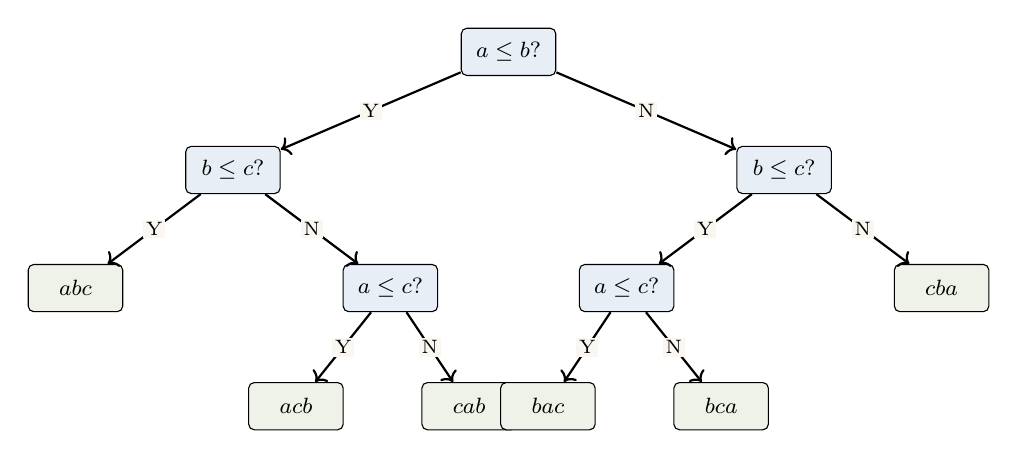
\begin{tikzpicture}[
    every node/.style={font=\footnotesize},
    cmp/.style={draw, rounded corners=2pt, fill=ideaBack,
                minimum width=12mm, minimum height=6mm, inner sep=2pt},
    leaf/.style={draw, fill=defnBack, rounded corners=2pt,
                minimum width=12mm, minimum height=6mm, inner sep=2pt},
    elabel/.style={font=\scriptsize, midway, fill=pagebg, inner sep=1pt}
]
% Root
\node[cmp] (root) at (0, 4) {$a \le b$?};
% Level 1
\node[cmp] (l1) at (-3.5, 2.5) {$b \le c$?};
\node[cmp] (l2) at ( 3.5, 2.5) {$b \le c$?};
% Level 2
\node[leaf] (ll1) at (-5.5, 1) {$abc$};
\node[cmp]  (ll2) at (-1.5, 1) {$a \le c$?};
\node[cmp]  (lr1) at ( 1.5, 1) {$a \le c$?};
\node[leaf] (lr2) at ( 5.5, 1) {$cba$};
% Level 3 leaves
\node[leaf] (lll1) at (-2.7, -0.5) {$acb$};
\node[leaf] (lll2) at (-0.5, -0.5) {$cab$};
\node[leaf] (lrr1) at ( 0.5, -0.5) {$bac$};
\node[leaf] (lrr2) at ( 2.7, -0.5) {$bca$};
% Edges with labels
\draw[->, thick] (root) -- (l1) node[elabel]{Y};
\draw[->, thick] (root) -- (l2) node[elabel]{N};
\draw[->, thick] (l1) -- (ll1) node[elabel]{Y};
\draw[->, thick] (l1) -- (ll2) node[elabel]{N};
\draw[->, thick] (l2) -- (lr1) node[elabel]{Y};
\draw[->, thick] (l2) -- (lr2) node[elabel]{N};
\draw[->, thick] (ll2) -- (lll1) node[elabel]{Y};
\draw[->, thick] (ll2) -- (lll2) node[elabel]{N};
\draw[->, thick] (lr1) -- (lrr1) node[elabel]{Y};
\draw[->, thick] (lr1) -- (lrr2) node[elabel]{N};
\end{tikzpicture}
\end{center}

The leaves are the 6 permutations of $\{a, b, c\}$. The tree has
height 3, matching $\lceil \log_2 6 \rceil$. No 3-element
comparison sort can do better in the worst case: any tree with
fewer than 6 leaves would alias two distinct permutations and be
incorrect.

\subsection*{Comparison vs.\ non-comparison sorts}

\begin{notebox}[Comparison vs.\ non-comparison]
The $\Omega(n \log n)$ bound applies \emph{only} to sorts that use
key comparisons as their sole inspection of the input. Sorts that
look \emph{inside} keys --- counting sort treats the key as an
index, radix sort treats it as a sequence of digits, bucket sort
treats it as a numeric value to bin --- bypass the bound entirely.
This is not a contradiction: those sorts have access to extra
structure (key universe size, digit count, distribution
assumption) that a generic comparison sort does not. The
non-comparison sorts of \S13.6--\S13.7 trade that extra-knowledge
requirement for sub-$n \log n$ time.

The decision tree of a comparison sort fans out by 2 at each
internal node ($\le$ vs.\ $>$). A counting sort on an $n$-element
input over a key universe of size $k$ has access to $k$-way
branching at the indexing step, which is what lets it land
permutations in linear time when $k = O(n)$.
\end{notebox}

\section{13.1 Bubble Sort}

\subsection*{The algorithm}

\begin{defnbox}
\textbf{Bubble sort.} Repeatedly walk the array, comparing adjacent pairs and swapping if out of order. After each pass, the largest remaining unsorted element ``bubbles'' to the end.
\end{defnbox}

\begin{lstlisting}[basicstyle=\ttfamily\small,frame=single]
void bubbleSort(std::vector<int>& a) {
    int n = a.size();
    for (int i = 0; i < n - 1; ++i) {
        for (int j = 0; j < n - i - 1; ++j) {
            if (a[j] > a[j + 1])
                std::swap(a[j], a[j + 1]);
        }
    }
}
\end{lstlisting}

The inner loop shrinks each pass because the last $i$ elements are already in their final position.

\subsection*{Cost}

\begin{itemize}[leftmargin=*]
    \item Best case (already sorted): still $O(n^2)$ comparisons in the plain version. An optimization: short-circuit when an entire pass made no swaps, giving $O(n)$ best case.
    \item Average: $O(n^2)$.
    \item Worst case (reverse sorted): $O(n^2)$ comparisons, $O(n^2)$ swaps.
    \item Space: $O(1)$.
    \item Stable: yes (equal elements never swap past each other).
\end{itemize}

\begin{notebox}[Bubble sort vs.\ the lower bound of \S13.0]
Bubble sort's $O(n^2)$ average and worst-case cost is a long way
above the comparison-sort lower bound of $\Omega(n \log n)$ from
\S13.0 --- bubble is one of the worst-performing comparison sorts
that still gets the answer right. The chapter-3 sorts
(insertion / selection / merge) sit at the same $O(n^2)$ ceiling
(insertion / selection) or at the optimal $O(n \log n)$ bound
(merge); ch.~7's heapsort also achieves $O(n \log n)$. So the
ladder runs: bubble / insertion / selection at the bottom
($O(n^2)$); merge / heap / introsort / Timsort / pdqsort at the
optimal floor ($O(n \log n)$); counting / radix / bucket below the
floor for suitable data. The chapter-13 closing decision table in
\S13.9 collects all of these by problem.
\end{notebox}

\subsection*{Why you'll never use bubble sort}

\begin{warnbox}
Bubble sort is a \textbf{teaching tool}, nothing more. For any real data: \texttt{std::sort} (introsort), \texttt{std::stable\_sort} (merge sort), or a radix/bucket sort for integers. Bubble sort's $O(n^2)$ worst case on large inputs is not just slow -- it's catastrophically slow. $n = 10^6$ is $10^{12}$ operations, roughly an hour of CPU time. A real sort does the same job in milliseconds.
\end{warnbox}

\begin{notebox}
The one defense of bubble sort: its best case with the short-circuit optimization is $O(n)$, matching insertion sort. For nearly-sorted data, it's not terrible. But insertion sort is better on the same workload and easier to reason about, so even that niche has a better answer. (Insertion / selection / merge sort live in ch.~3; heapsort in ch.~7. \S13.9's decision table collects every option side-by-side.)
\end{notebox}

\subsection*{What bubble sort is good for}

\begin{itemize}[leftmargin=*]
    \item Teaching the concept of an in-place comparison sort.
    \item Interview questions about algorithmic complexity.
    \item Tiny inputs ($n \leq 20$) where the constant factor is irrelevant.
    \item Hardware sorting networks, where adjacent-pair compare-and-swap is the primitive operation.
\end{itemize}

\section{13.2 Quickselect}

\subsection*{The problem}

\begin{defnbox}
\textbf{$k$-th smallest element.} Given an array and an integer $k$, return the $k$-th smallest value. For $k=0$, the minimum; for $k = n-1$, the maximum; for $k = n/2$, the median.
\end{defnbox}

The naive solution: sort, return \texttt{a[k]}. That's $O(n \log n)$. Quickselect does it in $O(n)$ average time \emph{without} fully sorting.

\subsection*{The insight}

Quickselect borrows Quicksort's partition routine -- the one that picks a pivot, puts smaller elements to the left, larger to the right, and returns the pivot's final position.

\begin{ideabox}
\textbf{Quicksort recurses on both sides; quickselect recurses on only the side that contains the $k$-th element.} That cuts the total work from $O(n \log n)$ to $O(n)$ on average, because the unused half of each partition is discarded.
\end{ideabox}

\subsection*{Algorithm}

\begin{lstlisting}[basicstyle=\ttfamily\small,frame=single]
int partition(std::vector<int>& a, int lo, int hi) {
    int pivot = a[(lo + hi) / 2];
    int i = lo - 1, j = hi + 1;
    while (true) {
        do { ++i; } while (a[i] < pivot);
        do { --j; } while (a[j] > pivot);
        if (i >= j) return j;
        std::swap(a[i], a[j]);
    }
}

int quickselect(std::vector<int>& a, int lo, int hi, int k) {
    if (lo >= hi) return a[lo];
    int p = partition(a, lo, hi);
    if (k <= p) return quickselect(a, lo, p, k);
    return quickselect(a, p + 1, hi, k);
}
\end{lstlisting}

\subsection*{Cost}

\begin{itemize}[leftmargin=*]
    \item \textbf{Average}: $O(n)$. Partition costs $n$; the next recursion is on $n/2$; then $n/4$; \ldots total $n + n/2 + n/4 + \ldots = O(n)$ by geometric sum.
    \item \textbf{Worst}: $O(n^2)$, same as naive quicksort, when pivots are consistently bad.
    \item \textbf{Median-of-medians} gives $O(n)$ worst-case selection, but the constant is large; in practice quickselect with a random or median-of-three pivot is faster.
\end{itemize}

\subsection*{Median-of-medians for worst-case $O(n)$ selection}

The median-of-medians algorithm (Blum, Floyd, Pratt, Rivest,
Tarjan, 1973; CLRS \S9.3) gives \emph{worst-case} $O(n)$
selection by computing a pivot guaranteed to be ``good enough'' on
every input. The construction:

\begin{enumerate}[leftmargin=*]
    \item Split the input into $\lceil n / 5 \rceil$ groups of 5
          consecutive elements (the last group may have fewer
          than 5).
    \item Sort each group in $O(1)$ time (5 elements: at most
          7 comparisons by an optimal 5-element sorting network).
          The middle of each sorted group is that group's median.
    \item \emph{Recursively} call median-of-medians on the
          collected $\lceil n/5 \rceil$ group-medians to find
          their median --- call it $M$.
    \item Use $M$ as the pivot for the standard quickselect
          partition step.
\end{enumerate}

The pivot $M$ is greater than at least
$3 \lceil n/10 \rceil - 6$ elements and less than at least
$3 \lceil n/10 \rceil - 6$ elements (each of the $\lceil n/10 \rceil$
groups whose median is below $M$ contributes at least 3 elements
below $M$). This guarantees that every recursive call shrinks the
problem by at least a $7/10$ factor in the worst case. The
recurrence
$T(n) \le T(n/5) + T(7n/10) + O(n)$
solves to $T(n) = O(n)$ because $1/5 + 7/10 = 9/10 < 1$.

\begin{notebox}[\texttt{std::nth\_element} guarantees]
The C++ standard's \texttt{std::nth\_element} is required to run
in average linear time but does not guarantee worst-case linear
time. libstdc++ implements it as introselect: quickselect with a
recursion-depth fallback to median-of-medians (analogous to
\texttt{std::sort}'s introsort fallback to heapsort). In practice
the recursion-depth fallback is rarely hit on production data ---
random pivots make the worst case astronomically unlikely --- but
the fallback exists so the worst case is bounded.
\end{notebox}

\subsection*{C++ standard library}

You don't have to write quickselect yourself -- C++ gives it to you:

\begin{lstlisting}[basicstyle=\ttfamily\small,frame=single]
#include <algorithm>
// Rearranges [begin, end) so nth is the element that would be at
// position n in a fully sorted range. Everything before nth is <=,
// everything after is >=. Average O(n).
std::nth_element(a.begin(), a.begin() + k, a.end());
int kthSmallest = a[k];
\end{lstlisting}

\begin{ideabox}
\texttt{std::nth\_element} is the correct answer to ``what's the median / top-$k$ / $k$-th percentile'' in any interview or real codebase. It's linear time, in place, and a single line of code. Reach for it before thinking harder.
\end{ideabox}

\begin{examplebox}[{Median of $[3, 1, 4, 1, 5, 9, 2, 6]$ via quickselect}]
Input: $a = [3, 1, 4, 1, 5, 9, 2, 6]$, $n = 8$, target
$k = n/2 = 4$ (the upper median --- the 5th-smallest, 0-indexed
position 4).

Sorted: $[1, 1, 2, 3, 4, 5, 6, 9]$ so the answer is 4.

\textbf{Trace using the listing above's Hoare partition with
midpoint pivot:}

\textbf{Call 1:} \texttt{quickselect(a, 0, 7, 4)}.
Pivot = $a[(0+7)/2] = a[3] = 1$. Hoare's two-pointer scan: $i$
advances from $-1$ while $a[i] < 1$ (no, $a[0] = 3 \ge 1$), $j$
retreats from $8$ while $a[j] > 1$ ($a[7] = 6, a[6] = 2$, then
$a[5] = 9, a[4] = 5, a[3] = 1$, stop). $i = 0, j = 3$. Since
$i < j$, swap $a[0] \leftrightarrow a[3]$:
$a = [1, 1, 4, 3, 5, 9, 2, 6]$. Continue: $i$ advances to 1
($a[1] = 1$, not less than pivot, stop), $j$ retreats to 0
($a[2] = 4, a[1] = 1$, stop). Now $i = 1 \ge j = 1$. Return
$j = 1$. Pivot's final position is 1; $k = 4 > 1$, so recurse
right: \texttt{quickselect(a, 2, 7, 4)}.

\textbf{Call 2:} \texttt{quickselect(a, 2, 7, 4)} on subarray
$[4, 3, 5, 9, 2, 6]$. Pivot = $a[(2+7)/2] = a[4] = 5$. After
partition: subarray becomes $[4, 3, 2, 5, 9, 6]$ (or similar
depending on the exact swap order; pivot 5 lands at position 5).
Hoare scan returns $j = 5$. $k = 4 \le 5$, recurse left:
\texttt{quickselect(a, 2, 5, 4)}.

\textbf{Call 3:} \texttt{quickselect(a, 2, 5, 4)} on subarray
$[4, 3, 2, 5]$. Pivot = $a[(2+5)/2] = a[3] = 3$. After partition:
$[2, 3, 4, 5]$ with pivot at position 3. Returns $j = 3$.
$k = 4 > 3$, recurse right: \texttt{quickselect(a, 4, 5, 4)}.

\textbf{Call 4:} \texttt{quickselect(a, 4, 5, 4)} on $[4, 5]$.
Pivot = $a[(4+5)/2] = a[4] = 4$. Partition is no-op
(already in order); returns $j = 4$. $k = 4 \le 4$, recurse
left: \texttt{quickselect(a, 4, 4, 4)} returns $a[4] = 4$.

\textbf{Result:} the 5th-smallest (0-indexed position 4) is
\textbf{4}. The total comparison work was $O(n)$ as expected:
calls processed subarrays of sizes $8, 6, 4, 2$, summing under
the geometric series $\le 2n$.
\end{examplebox}

\subsection*{Applications}

\begin{itemize}[leftmargin=*]
    \item \textbf{Median / percentile computation.}
    \item \textbf{Top-$k$ queries.} After \texttt{nth\_element}, the first $k$ entries are the top-$k$ (unsorted). If you need them sorted, sort just that prefix.
    \item \textbf{Machine learning}: quickselect-based k-nearest-neighbor scoring.
    \item \textbf{Streaming statistics}: approximate quantiles via repeated quickselect.
\end{itemize}

\section{13.3 Bucket Sort}

\subsection*{The idea}

\begin{defnbox}
\textbf{Bucket sort.} Distribute values into $K$ buckets based on a range partition, sort each bucket with another algorithm, concatenate. $O(n)$ average when values are uniformly distributed.
\end{defnbox}

This is a \textbf{non-comparison sort} -- it exploits numerical structure of the values to beat the $\Omega(n \log n)$ comparison-sort lower bound (\S13.0).

\begin{notebox}[Scope of \S13.3 vs.\ \S13.6 / \S13.7]
This section covers \emph{bucket sort proper} (range-partition into
$K$ buckets, per-bucket comparison sort, concatenate). Two
sibling sorts in the non-comparison family get their own sections
later: \emph{counting sort} (bucket sort degenerated to one bucket
per key value, no per-bucket sort needed) lives in \S13.6, and
\emph{radix sort} (iterated counting sort, one pass per digit)
lives in \S13.7. The closing notebox of this section sketches the
family-tree relationship; the full algorithms come later.
\end{notebox}

\subsection*{Algorithm}

Given non-negative numbers up to some max value $M$:

\begin{enumerate}[leftmargin=*]
    \item Create $K$ buckets. Bucket $i$ holds values in $[i \cdot M/K, (i+1) \cdot M/K)$.
    \item For each element $x$, compute \texttt{bucket = floor(x * K / (M + 1))} and append $x$ to that bucket.
    \item Sort each bucket (insertion sort or any other; each bucket is small).
    \item Concatenate buckets in order.
\end{enumerate}

\begin{lstlisting}[basicstyle=\ttfamily\small,frame=single]
void bucketSort(std::vector<int>& a, int K) {
    if (a.empty()) return;
    int maxV = *std::max_element(a.begin(), a.end());
    std::vector<std::vector<int>> buckets(K);

    for (int x : a) {
        int idx = (long long)x * K / (maxV + 1);
        buckets[idx].push_back(x);
    }

    a.clear();
    for (auto& b : buckets) {
        std::sort(b.begin(), b.end());
        a.insert(a.end(), b.begin(), b.end());
    }
}
\end{lstlisting}

\subsection*{Cost}

Let $n$ be the array size and $K$ the bucket count.
\begin{itemize}[leftmargin=*]
    \item \textbf{Distribution pass}: $O(n)$.
    \item \textbf{Per-bucket sort}: if values are uniform, each bucket has $\approx n/K$ elements. Sorting each with $O(m^2)$ insertion sort gives total $K \cdot (n/K)^2 = n^2/K$. With $K = n$, this is $O(n)$.
    \item \textbf{Concatenate}: $O(n + K)$.
    \item \textbf{Total (uniform distribution, $K = n$)}: $O(n)$.
    \item \textbf{Worst case (all elements in one bucket)}: $O(n^2)$.
\end{itemize}

\begin{warnbox}
Bucket sort's $O(n)$ is \emph{contingent on distribution}. If all your values cluster in a narrow range (e.g., 100 random integers between 1 and $10^9$), bucket sort degenerates: 99 empty buckets, one bucket with everything. You're paying for $K$ buckets to do nothing. Use bucket sort only when you know the data is roughly uniform over a known range.
\end{warnbox}

\subsection*{Related algorithms}

\begin{itemize}[leftmargin=*]
    \item \textbf{Counting sort}: degenerate bucket sort where each bucket holds exactly one value. $O(n + M)$ time, $O(M)$ space. Perfect for small-range integers. Full treatment in \S13.6.
    \item \textbf{Radix sort}: iterate counting sort on each digit. $O(d(n + b))$ for $d$-digit numbers in base $b$. Used in database sorts, GPU sorts, and networking. Full treatment in \S13.7.
    \item \textbf{Pigeonhole sort}: counting sort by another name, when value range $=$ number of elements.
\end{itemize}

\begin{ideabox}
\textbf{The $n \log n$ barrier only applies to comparison sorts.} Any sort that uses numeric / string structure of its inputs -- bucket, radix, counting -- can beat it for suitable data. Production string sorting (timsort in Python, dpqsort in Java) is comparison-based; production integer sorting (std::sort in libstdc++ at large sizes) can fall through to radix for speed.
\end{ideabox}

\section{13.4 List Data Structure}

\subsection*{The idiom}

A linked list (ch.~4) can be represented in two ways:

\begin{itemize}[leftmargin=*]
    \item \textbf{Just a head pointer} (and maybe a tail pointer), held in local variables or as member fields.
    \item \textbf{A wrapper container} -- a \texttt{List} struct that owns \texttt{head}, \texttt{tail}, and maybe \texttt{size}. Functions take a \texttt{List*} instead of a raw head pointer.
\end{itemize}

\begin{lstlisting}[basicstyle=\ttfamily\small,frame=single]
// Approach 1: just nodes.
struct Node { int data; Node* next; };
Node* head = nullptr;
Node* tail = nullptr;
int size = 0;

// Approach 2: list wrapper.
struct List {
    Node* head = nullptr;
    Node* tail = nullptr;
    int size = 0;
};

void listPushBack(List* lst, int data) {
    Node* n = new Node{data, nullptr};
    if (!lst->head) lst->head = n;
    else            lst->tail->next = n;
    lst->tail = n;
    ++lst->size;
}
\end{lstlisting}

\subsection*{Why wrap?}

\begin{ideabox}
The wrapper exists so that list-manipulating functions take \emph{one} parameter instead of three (head, tail, size). More importantly, operations like ``insert at tail'' or ``get length'' become $O(1)$ because the struct already knows what the naked-node version would have to recompute.
\end{ideabox}

\begin{center}
\begin{tabular}{lll}
\hline
Operation & Head-only list & Wrapped list \\
\hline
Insert at head & $O(1)$ & $O(1)$ \\
Insert at tail & $O(n)$ (walk to end) & $O(1)$ (tail ptr) \\
Get size & $O(n)$ or maintained externally & $O(1)$ (cached) \\
Pass to function & 3 args (head, tail, size) & 1 arg (\texttt{List*}) \\
\hline
\end{tabular}
\end{center}

\subsection*{Why not just use \texttt{std::list}?}

\begin{warnbox}
In C++, \texttt{std::list} is the wrapper-style doubly-linked list and you should use it unless you have a specific reason not to. Writing your own list is a pedagogical exercise; in production, \texttt{std::list} (or \texttt{std::forward\_list} for singly-linked) is tested, debuggers know how to render it, and you don't leak memory on exception. The ``list data structure'' the textbook describes is reinventing \texttt{std::list}.
\end{warnbox}

\begin{notebox}[\texttt{std::list} vs.\ \texttt{std::forward\_list}]
The C++ STL ships \emph{two} linked-list containers, mirroring the
two flavours covered in ch.~4:
\begin{itemize}[leftmargin=*]
    \item \texttt{std::list} (since C++98) is a \emph{doubly-linked
          list} with head and tail sentinels: $O(1)$
          \texttt{push\_front} / \texttt{pop\_front} /
          \texttt{push\_back} / \texttt{pop\_back}, $O(1)$
          \texttt{size()} (cached since C++11), $O(1)$ insertion
          and deletion at any iterator. Iterator invariants are
          stable: an iterator to a node is valid for that node's
          entire lifetime, not just until the next mutation.
    \item \texttt{std::forward\_list} (since C++11) is a
          \emph{singly-linked list} with a head-only sentinel:
          $O(1)$ \texttt{push\_front} / \texttt{pop\_front},
          $O(n)$ tail operations (no tail pointer, by design),
          \emph{no} \texttt{size()} method (would require $O(n)$
          traversal --- C++11 left it off rather than cache it,
          since the use case for \texttt{forward\_list} is
          ``smaller per-node footprint when you don't need cached
          size or doubly-linked traversal'').
\end{itemize}
The naming follows the same pattern as
\texttt{std::set} / \texttt{std::unordered\_set} (ch.~12): the
unqualified name is the more featureful default.
\end{notebox}

\subsection*{When linked lists are the wrong answer}

Even with a nice wrapper, linked lists are frequently worse than \texttt{std::vector} (dynamic array):

\begin{itemize}[leftmargin=*]
    \item Cache locality: array elements are contiguous, list nodes scattered across the heap.
    \item Memory overhead: each node has a \texttt{next} pointer, often doubling memory vs.\ raw values.
    \item Random access: $O(n)$ for list, $O(1)$ for array.
    \item Iteration: much slower on a list due to cache misses on every \texttt{next}.
\end{itemize}

Use a linked list when you need cheap insertion/deletion at interior points with existing iterators, or when you're building something that requires pointer stability (e.g., an LRU cache with external references). Otherwise, default to \texttt{std::vector}.

\section{13.5 Circular Lists}

\subsection*{The definition}

\begin{defnbox}
\textbf{Circular linked list.} A linked list (ch.~4) where the tail's \texttt{next} pointer points back to the head, not \texttt{nullptr}. Traversal wraps forever unless explicitly bounded.
\end{defnbox}

\begin{lstlisting}[basicstyle=\ttfamily\small,frame=single]
// Singly-linked circular
struct Node { int data; Node* next; };
// Last node's next points back to head.

// Doubly-linked circular (most common in practice)
struct DNode { int data; DNode* prev; DNode* next; };
// Last node's next -> head; head's prev -> last node.
\end{lstlisting}

\subsection*{Traversal}

The key trick: stop when you come back to the start, not when you hit \texttt{nullptr}.

\begin{lstlisting}[basicstyle=\ttfamily\small,frame=single]
void traverseCircular(Node* head) {
    if (!head) return;
    Node* cur = head;
    do {
        visit(cur);
        cur = cur->next;
    } while (cur != head);
}
\end{lstlisting}

\begin{warnbox}
\textbf{Use do-while, not while.} A regular \texttt{while (cur != head)} skips the head on the first iteration because we start at head and the condition fails immediately. The do-while runs the body first, then checks the condition.
\end{warnbox}

\subsection*{Why circular lists exist}

\begin{itemize}[leftmargin=*]
    \item \textbf{Round-robin scheduling.} OS schedulers cycle through ready processes; each yield pops one and reappends it at the end. A circular list gives O(1) ``next process'' and O(1) append.
    \item \textbf{Music players on ``repeat all.''} Queue is a circular list of tracks.
    \item \textbf{Ring buffers} (logically circular, though usually array-based for cache locality).
    \item \textbf{Josephus problem} and other classic cyclic-elimination algorithms -- naturally circular.
    \item \textbf{Token-passing networks.} Token Ring Ethernet was literally a circular list of nodes; each station had one successor.
    \item \textbf{Doubly-linked circular lists with a sentinel} give branch-free insert/delete at any position.
\end{itemize}

\subsection*{Sentinel trick for doubly-linked circular lists}

A \emph{sentinel} node -- a dummy that's never ``real'' data but completes the circle -- removes the ``is this node the head / tail'' special cases:

\begin{lstlisting}[basicstyle=\ttfamily\small,frame=single]
struct DNode { int data; DNode* prev; DNode* next; };

struct CircularList {
    DNode sentinel;   // sentinel.next = head, sentinel.prev = tail
    CircularList() { sentinel.prev = sentinel.next = &sentinel; }
};

// Insert n before 'where' -- no null checks needed.
void insertBefore(DNode* where, DNode* n) {
    n->next = where;
    n->prev = where->prev;
    where->prev->next = n;
    where->prev = n;
}

// Remove n -- no null checks needed.
void remove(DNode* n) {
    n->prev->next = n->next;
    n->next->prev = n->prev;
}
\end{lstlisting}

\begin{center}
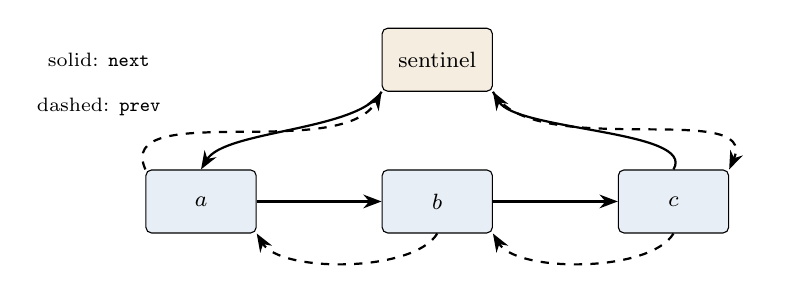
\begin{tikzpicture}[
    every node/.style={font=\footnotesize},
    snode/.style={draw, rounded corners=2pt, fill=warnBack,
                  minimum width=14mm, minimum height=8mm, inner sep=2pt},
    dnode/.style={draw, rounded corners=2pt, fill=ideaBack,
                  minimum width=14mm, minimum height=8mm, inner sep=2pt},
    arr/.style={->, >=Stealth, thick}
]
% Sentinel at top-center
\node[snode] (S) at (0, 1.6) {sentinel};
% Three real data nodes around it, circular
\node[dnode] (A) at (-3, -0.2) {$a$};
\node[dnode] (B) at ( 0, -0.2) {$b$};
\node[dnode] (C) at ( 3, -0.2) {$c$};
% Forward (next) arrows on top side
\draw[arr] (S.south west) .. controls ($(S.south west)+(-0.3,-0.5)$) and ($(A.north)+(0.3,0.5)$) .. (A.north);
\draw[arr] (A.east) -- (B.west);
\draw[arr] (B.east) -- (C.west);
\draw[arr] (C.north) .. controls ($(C.north)+(0.3,0.5)$) and ($(S.south east)+(0.3,-0.5)$) .. (S.south east);
% Backward (prev) arrows on bottom side
\draw[arr, dashed] (S.south east) .. controls ($(S.south east)+(0.5,-0.9)$) and ($(C.north east)+(0.4,0.9)$) .. (C.north east);
\draw[arr, dashed] (C.south) .. controls ($(C.south)+(-0.3,-0.5)$) and ($(B.south east)+(0.3,-0.5)$) .. (B.south east);
\draw[arr, dashed] (B.south) .. controls ($(B.south)+(-0.3,-0.5)$) and ($(A.south east)+(0.3,-0.5)$) .. (A.south east);
\draw[arr, dashed] (A.north west) .. controls ($(A.north west)+(-0.4,0.9)$) and ($(S.south west)+(-0.5,-0.9)$) .. (S.south west);
% Legend
\node[font=\scriptsize] at (-4.3, 1.6) {solid: \texttt{next}};
\node[font=\scriptsize] at (-4.3, 1.0) {dashed: \texttt{prev}};
\end{tikzpicture}
\end{center}

The sentinel is always present, even when the list is logically
empty (then \texttt{sentinel.next == sentinel.prev == \&sentinel}).
There is no ``\texttt{head == nullptr}'' branch in
\texttt{insertBefore} / \texttt{remove} --- the sentinel guarantees
both \texttt{prev} and \texttt{next} are non-null for every real
node, and operations on the sentinel itself are well-defined.

\begin{ideabox}
The sentinel technique eliminates all ``empty list'' and ``at the head'' edge cases. Insert/remove are six pointer writes with no branching. The Linux kernel's \texttt{list\_head} uses exactly this structure, and the design has been copied into countless production codebases -- it's one of the most elegant tricks in systems programming.
\end{ideabox}

\subsection*{Traversal in reverse (doubly-linked)}

Mirror of the forward case -- walk \texttt{prev} pointers from any starting point until you return:

\begin{lstlisting}[basicstyle=\ttfamily\small,frame=single]
void traverseReverseCircular(DNode* tail) {
    if (!tail) return;
    DNode* cur = tail;
    do {
        visit(cur);
        cur = cur->prev;
    } while (cur != tail);
}
\end{lstlisting}

\section{13.6 Counting sort}

\subsection*{The idea}

\begin{defnbox}
\textbf{Counting sort.} A linear-time stable sort for keys in
$[0, k)$. Counts the occurrences of each key value, computes a
prefix-sum to find each key's starting output position, then
places each input element into the output array in a single
right-to-left pass. Runs in $O(n + k)$ time and $O(n + k)$ space.
\end{defnbox}

Counting sort sidesteps the comparison-sort lower bound of \S13.0
by treating each key as an array index rather than as something to
compare. The price: it only works when keys are non-negative
integers in a known small-ish range.

\subsection*{Algorithm}

Given input $A[0 \dots n-1]$ with each $A[i] \in [0, k)$:

\begin{enumerate}[leftmargin=*]
    \item \textbf{Count.} Allocate
          $C[0 \dots k-1]$ initialised to zero. Scan $A$ once;
          for each $A[i]$, increment $C[A[i]]$. Now $C[v]$ is the
          number of input elements equal to $v$.
    \item \textbf{Prefix sum.} Replace $C$ with its running sum:
          $C[v] \leftarrow C[v] + C[v-1]$ for $v$ from 1 to $k-1$.
          Now $C[v]$ is the number of input elements $\le v$, which
          is also one past the last position where a $v$ should
          land in the output.
    \item \textbf{Place.} Allocate output $B[0 \dots n-1]$.
          Iterate $i$ from $n-1$ down to $0$ (\emph{right-to-left}
          for stability); for each $A[i]$, set
          $C[A[i]] \leftarrow C[A[i]] - 1$, then
          $B[C[A[i]]] \leftarrow A[i]$.
\end{enumerate}

\begin{lstlisting}[basicstyle=\ttfamily\small,frame=single]
// Stable counting sort. Keys must satisfy 0 <= a[i] < k.
void countingSort(std::vector<int>& a, int k) {
    int n = a.size();
    if (n == 0) return;
    std::vector<int> C(k, 0);
    std::vector<int> B(n);

    // 1. Count.
    for (int i = 0; i < n; ++i) ++C[a[i]];

    // 2. Prefix sum: C[v] = number of inputs <= v.
    for (int v = 1; v < k; ++v) C[v] += C[v - 1];

    // 3. Place right-to-left for stability.
    for (int i = n - 1; i >= 0; --i) {
        --C[a[i]];
        B[C[a[i]]] = a[i];
    }

    a = std::move(B);
}
\end{lstlisting}

\subsection*{Cost}

\begin{itemize}[leftmargin=*]
    \item \textbf{Time}: $O(n + k)$. Three linear scans of size
          $n$, $k$, $n$.
    \item \textbf{Space}: $O(n + k)$. The count array $C$ has
          size $k$; the output array $B$ has size $n$.
    \item \textbf{Stable}: yes. The right-to-left placement
          guarantees that two equal elements preserve their input
          order. (Going left-to-right would reverse them ---
          this is the most common counting-sort bug.)
    \item \textbf{In-place}: no. Counting sort needs $O(n + k)$
          auxiliary space.
\end{itemize}

\begin{ideabox}[When counting sort beats quicksort]
Counting sort outperforms quicksort exactly when $k = O(n)$ ---
i.e.\ the key universe is at most linear in the input size. At
$k = n$, counting sort is $O(n)$ vs.\ quicksort's
$O(n \log n)$. At $k = n^2$, counting sort costs $O(n^2)$ for
the prefix-sum scan alone --- worse than \emph{any} comparison
sort. The break-even crossover is roughly $k = n \log n$. As a
rule of thumb: counting sort beats comparison sorts when the key
universe is at most a few times the input size and you can afford
the $O(k)$ memory for the count array.
\end{ideabox}

\subsection*{Stability proof}

\textbf{Claim.} Counting sort with right-to-left placement is
stable: for $i < j$ with $A[i] = A[j]$, the output places $A[i]$
before $A[j]$.

\textbf{Proof sketch.} The right-to-left placement loop processes
$A[j]$ first (since $j > i$), decrements $C[A[j]]$, and writes
$A[j]$ to position $C[A[j]]$. When the loop later reaches $A[i]$,
$C[A[i]]$ has been decremented at least once (by the $A[j]$
write), so $A[i]$ writes to a smaller index --- i.e.\ to the left
of $A[j]$ in the output. Stability holds for any equal-key pair.

\subsection*{Worked layout: counting array $\to$ output}

\begin{center}
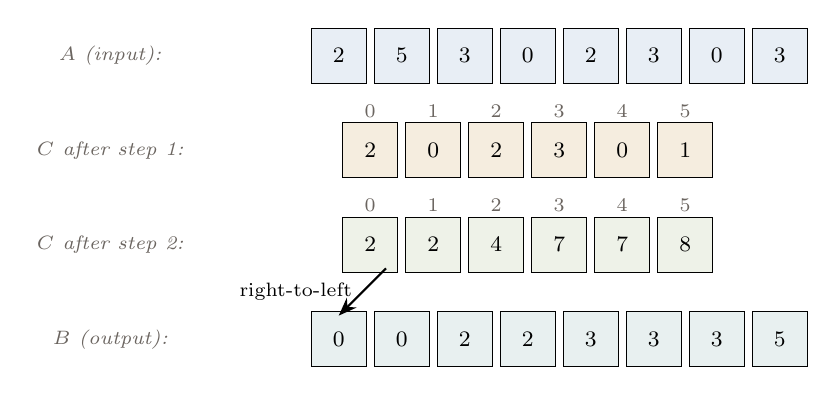
\begin{tikzpicture}[
    every node/.style={font=\footnotesize},
    cell/.style={draw, rectangle, minimum width=7mm, minimum height=7mm,
                 inner sep=0pt},
    lab/.style={font=\scriptsize\itshape, mutedtext},
    arr/.style={->, >=Stealth, thick}
]
% Input row
\node[lab] at (-4.5, 2.0) {$A$ (input):};
\foreach \x/\v in {0/2, 1/5, 2/3, 3/0, 4/2, 5/3, 6/0, 7/3} {
    \node[cell, fill=ideaBack] at (\x*0.8 - 1.6, 2.0) {\v};
}
% Count array C after step 1
\node[lab] at (-4.5, 0.8) {$C$ after step 1:};
\foreach \v/\c in {0/2, 1/0, 2/2, 3/3, 4/0, 5/1} {
    \node[cell, fill=warnBack] at (\v*0.8 - 1.2, 0.8) {\c};
    \node[font=\scriptsize, mutedtext] at (\v*0.8 - 1.2, 1.3) {\v};
}
% Count array C after prefix sum
\node[lab] at (-4.5, -0.4) {$C$ after step 2:};
\foreach \v/\c in {0/2, 1/2, 2/4, 3/7, 4/7, 5/8} {
    \node[cell, fill=defnBack] at (\v*0.8 - 1.2, -0.4) {\c};
    \node[font=\scriptsize, mutedtext] at (\v*0.8 - 1.2, 0.1) {\v};
}
% Output row B
\node[lab] at (-4.5, -1.6) {$B$ (output):};
\foreach \x/\v in {0/0, 1/0, 2/2, 3/2, 4/3, 5/3, 6/3, 7/5} {
    \node[cell, fill=exBack] at (\x*0.8 - 1.6, -1.6) {\v};
}
% Annotation arrow from C[step2] to B
\draw[arr] (-1.0, -0.7) -- (-1.6, -1.3) node[midway, left, font=\scriptsize] {right-to-left};
\end{tikzpicture}
\end{center}

The picture above sorts $A = [2, 5, 3, 0, 2, 3, 0, 3]$ in three
phases: the count vector $C$ tallies each key value (top: two
0s, no 1s, two 2s, three 3s, no 4s, one 5); the prefix sum
($C \leftarrow$ running sum) gives the position one past where
each key class ends in $B$; the right-to-left placement step
walks the input backward and stamps each element into its
final slot, decrementing $C$ as it goes.

\begin{examplebox}[{Counting sort on $[2, 5, 3, 0, 2, 3, 0, 3]$}]
$A = [2, 5, 3, 0, 2, 3, 0, 3]$, $n = 8$, $k = 6$ (keys in $[0, 6)$).

\textbf{Step 1 (count).}
$C = [\,2,\,0,\,2,\,3,\,0,\,1\,]$ --- two 0s, no 1s, two 2s, three
3s, no 4s, one 5.

\textbf{Step 2 (prefix sum).}
$C = [\,2,\,2,\,4,\,7,\,7,\,8\,]$. Each $C[v]$ is now ``one past
the last position where a $v$ goes.'' For example, the 3s end at
output position 7, so $B[4..6]$ will hold the three 3s.

\textbf{Step 3 (right-to-left placement).}
\begin{itemize}[leftmargin=*]
    \item $i = 7$: $A[7] = 3$. $C[3] \to 6$, $B[6] = 3$.
    \item $i = 6$: $A[6] = 0$. $C[0] \to 1$, $B[1] = 0$.
    \item $i = 5$: $A[5] = 3$. $C[3] \to 5$, $B[5] = 3$.
    \item $i = 4$: $A[4] = 2$. $C[2] \to 3$, $B[3] = 2$.
    \item $i = 3$: $A[3] = 0$. $C[0] \to 0$, $B[0] = 0$.
    \item $i = 2$: $A[2] = 3$. $C[3] \to 4$, $B[4] = 3$.
    \item $i = 1$: $A[1] = 5$. $C[5] \to 7$, $B[7] = 5$.
    \item $i = 0$: $A[0] = 2$. $C[2] \to 2$, $B[2] = 2$.
\end{itemize}

\textbf{Result.} $B = [0, 0, 2, 2, 3, 3, 3, 5]$, sorted and
stable. Total work: $n = 8$ for the count pass, $k = 6$ for the
prefix-sum pass, $n = 8$ for placement.
\end{examplebox}

\subsection*{Use cases}

\begin{itemize}[leftmargin=*]
    \item \textbf{Pre-pass for radix sort.} Each digit pass of
          radix sort is a counting sort on $k = b$ (the radix).
          \S13.7 fully exploits this.
    \item \textbf{Integer histograms in image processing.} Pixel
          intensities are 8-bit ($k = 256$); a counting-sort
          ``count'' phase \emph{is} the histogram, and the
          prefix-sum phase \emph{is} the cumulative
          distribution function used in histogram equalisation.
    \item \textbf{Database aggregations.} \texttt{GROUP BY} on a
          low-cardinality column (e.g.\ enum / boolean / status)
          is a counting sort: bucketise rows by group key in
          one pass.
    \item \textbf{Bucket sort sub-step.} When per-bucket sort in
          \S13.3 turns out to be on a small key universe,
          counting sort is what to reach for.
\end{itemize}

\section{13.7 Radix sort}

\subsection*{The idea}

\begin{defnbox}
\textbf{Radix sort.} Sort $d$-digit keys in base $b$ by repeating
a stable single-digit sort once per digit. The standard form is
\emph{LSD radix sort}: process digits from least-significant to
most-significant, with counting sort doing each digit pass.
Runs in $O(d(n + b))$ time and $O(n + b)$ space.
\end{defnbox}

Radix sort beats the comparison-sort lower bound when keys are
fixed-width: $O(d(n + b)) = O(n)$ if $d$ and $b$ are both
constants. For 32-bit integers with $b = 256$ ($d = 4$ byte
passes), that gives roughly $4 \cdot (n + 256) = O(n)$ work --- which is
why radix sort is the standard parallel sort on GPUs and the
go-to integer sort in production analytics engines.

\subsection*{LSD algorithm}

The crucial property: each digit pass must be a \emph{stable}
sort, and counting sort is stable by construction (\S13.6). So:

\begin{enumerate}[leftmargin=*]
    \item For digit position $p = 0, 1, \dots, d-1$ (from
          least-significant to most-significant):
          \begin{enumerate}
              \item Stable-counting-sort the array on the value
                    of digit $p$ (i.e.\ $\lfloor x / b^p \rfloor
                    \bmod b$ as the key for input $x$).
          \end{enumerate}
    \item After $d$ passes, the array is fully sorted.
\end{enumerate}

\begin{lstlisting}[basicstyle=\ttfamily\small,frame=single]
// LSD radix sort over non-negative integers in base b.
// d is the number of base-b digits sufficient to represent
// every input element.
void radixSortLSD(std::vector<int>& a, int b, int d) {
    int n = a.size();
    if (n == 0) return;
    std::vector<int> B(n);
    long long base = 1;  // = b^p

    for (int p = 0; p < d; ++p) {
        std::vector<int> C(b, 0);

        // Count digit-p occurrences.
        for (int i = 0; i < n; ++i) {
            int digit = (a[i] / base) % b;
            ++C[digit];
        }
        // Prefix sum.
        for (int v = 1; v < b; ++v) C[v] += C[v - 1];
        // Stable placement, right-to-left.
        for (int i = n - 1; i >= 0; --i) {
            int digit = (a[i] / base) % b;
            --C[digit];
            B[C[digit]] = a[i];
        }
        std::swap(a, B);
        base *= b;
    }
}
\end{lstlisting}

\subsection*{Cost}

\begin{itemize}[leftmargin=*]
    \item \textbf{Time}: $O(d(n + b))$. Each of the $d$ digit
          passes is a counting sort with parameters $n$ and $b$.
    \item \textbf{Space}: $O(n + b)$. One output buffer of size
          $n$ plus one count buffer of size $b$, reused across
          passes.
    \item \textbf{Stable}: yes. Stability of each digit pass is
          required for correctness.
    \item \textbf{In-place}: no, in the LSD form. (MSD variants
          can be made closer to in-place at the cost of recursion
          overhead.)
\end{itemize}

\subsection*{Base-vs-passes tradeoff}

\begin{ideabox}[Choosing the radix base $b$]
The cost $O(d(n + b))$ is minimised by trading $d$ against $b$.
For $w$-bit keys: $d = w / \log_2 b$ passes. Doubling $b$ halves
the number of passes but doubles the count-array size. The
practical sweet spot for 32-bit / 64-bit integer keys is
$b = 256$ --- one byte per pass, fits comfortably in L1 cache,
and the count array is $256 \cdot 4 = 1024$ bytes (or
$256 \cdot 8 = 2048$ bytes for 64-bit counters), tiny relative
to any production input. Production radix sorts (CUB on GPU,
Boost \texttt{spreadsort}, \texttt{ips4o}'s integer fast-path)
all use byte-per-pass radix.
\end{ideabox}

\subsection*{LSD passes on $[170, 45, 75, 90, 802, 24, 2, 66]$}

\begin{center}
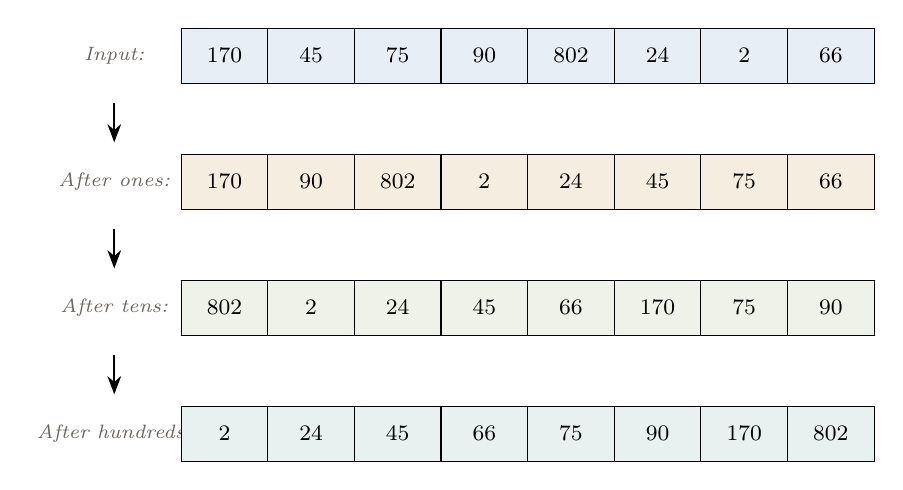
\begin{tikzpicture}[
    every node/.style={font=\footnotesize},
    cell/.style={draw, rectangle, minimum width=11mm, minimum height=7mm,
                 inner sep=1pt},
    lab/.style={font=\scriptsize\itshape, mutedtext},
    arr/.style={->, >=Stealth, thick}
]
% Initial
\node[lab] at (-5.6, 3.6) {Input:};
\foreach \x/\v in {0/170, 1/45, 2/75, 3/90, 4/802, 5/24, 6/2, 7/66} {
    \node[cell, fill=ideaBack] at (\x*1.1 - 4.2, 3.6) {\v};
}
% After 1s digit
\node[lab] at (-5.6, 2.0) {After ones:};
\foreach \x/\v in {0/170, 1/90, 2/802, 3/2, 4/24, 5/45, 6/75, 7/66} {
    \node[cell, fill=warnBack] at (\x*1.1 - 4.2, 2.0) {\v};
}
% After tens
\node[lab] at (-5.6, 0.4) {After tens:};
\foreach \x/\v in {0/802, 1/2, 2/24, 3/45, 4/66, 5/170, 6/75, 7/90} {
    \node[cell, fill=defnBack] at (\x*1.1 - 4.2, 0.4) {\v};
}
% After hundreds
\node[lab] at (-5.6, -1.2) {After hundreds:};
\foreach \x/\v in {0/2, 1/24, 2/45, 3/66, 4/75, 5/90, 6/170, 7/802} {
    \node[cell, fill=exBack] at (\x*1.1 - 4.2, -1.2) {\v};
}
% Vertical arrows between rows
\foreach \y in {3.0, 1.4, -0.2} {
    \draw[arr] (-5.6, \y) -- (-5.6, \y - 0.5);
}
\end{tikzpicture}
\end{center}

\begin{examplebox}[{LSD radix sort on $[170, 45, 75, 90, 802, 24, 2, 66]$}]
Input: $[170, 45, 75, 90, 802, 24, 2, 66]$. Base $b = 10$, three
digits sufficient ($d = 3$, since the max value 802 has 3 digits).

\textbf{Pass 1 --- ones digit.} The ones digits are
$0, 5, 5, 0, 2, 4, 2, 6$. Stable-counting-sort by ones digit:
\[
[170, \mathbf{90}, 802, 2, 24, 45, 75, 66]
\]
(170 keeps its position relative to 90 even though both have
ones-digit 0, because 170 came before 90 in the input. Then 802
and 2 with ones-digit 2 in input order; 24 alone with 4; 45
before 75 in input order with 5; 66 alone with 6.)

\textbf{Pass 2 --- tens digit.} Tens digits of the pass-1 output
are $7, 9, 0, 0, 2, 4, 7, 6$. Stable-counting-sort by tens digit:
\[
[802, 2, 24, 45, 66, 170, 75, 90]
\]
(802 and 2 have tens-digit 0 and stay in pass-1 order; 24, 45, 66
have tens 2, 4, 6; 170 and 75 both have tens-digit 7 and stay in
pass-1 order; 90 has tens-digit 9.)

\textbf{Pass 3 --- hundreds digit.} Hundreds digits of the
pass-2 output are $8, 0, 0, 0, 0, 1, 0, 0$. Stable-counting-sort
by hundreds digit:
\[
[2, 24, 45, 66, 75, 90, 170, 802]
\]
(All seven hundreds-digit-0 values stay in their pass-2 order;
170 has hundreds-digit 1; 802 has hundreds-digit 8.)

\textbf{Result.} Fully sorted in $d = 3$ passes, each pass an
$O(n + b)$ counting sort. Total work for $n = 8$, $b = 10$:
$3 \cdot (8 + 10) = 54$ key inspections plus the placement loops
--- linear in $n$.
\end{examplebox}

\subsection*{MSD radix sort and variable-length keys}

LSD radix sort requires every key to have the same number of
digits (or be left-padded with zeros). For variable-length keys
(strings of different lengths, IP addresses with optional
prefixes, etc.) the natural variant is \emph{MSD radix sort}:
process digits from \emph{most}-significant to least-significant,
recursing into each non-empty bucket.

\begin{itemize}[leftmargin=*]
    \item \textbf{Algorithm.} Bucket the input by the
          most-significant digit. Recursively radix-sort each
          non-empty bucket on the next digit. Concatenate buckets
          in MSD order.
    \item \textbf{Strings.} MSD radix on strings is the standard
          string-sort: bucket by first character, recurse on
          remaining suffix. The recursion bottoms out when a
          bucket has $\le 1$ string (already sorted) or when the
          suffix is empty.
    \item \textbf{When MSD beats LSD.} Variable-length keys (LSD
          would need padding); early-termination when most strings
          differ in their first few characters; cache locality
          (each MSD bucket fits in cache).
    \item \textbf{When LSD beats MSD.} Fixed-width keys
          (no recursion overhead); simpler code; no
          stack-depth bound.
\end{itemize}

\subsection*{Use cases}

\begin{itemize}[leftmargin=*]
    \item \textbf{GPU sorts.} Radix sort is the canonical parallel
          sort on GPUs (CUB, Thrust, NVIDIA's \texttt{cub::DeviceRadixSort}).
          The pattern is fully data-parallel: each digit pass is
          a histogram + prefix-scan + scatter, all with
          well-known GPU primitives.
    \item \textbf{Database engine sorts.} PostgreSQL's
          \texttt{ORDER BY} on integer / fixed-width keys; BigQuery
          / Snowflake / DuckDB column-store sorts.
    \item \textbf{Spotify / streaming-recommendation pipelines.}
          Sort-by-user-id or sort-by-track-id at the petabyte
          scale uses radix because integer key universes are
          natural and the parallelism is trivial.
    \item \textbf{Network packet processing.} Sort by source IP
          / destination IP / 5-tuple flow key is a fixed-width
          radix sort, used in DPDK and packet-capture pipelines.
\end{itemize}

\section{13.8 Production hybrid sorts}

The lower bound of \S13.0 says no comparison sort beats
$O(n \log n)$ in the worst case. But real data is not the
worst case --- it has structure (already-sorted runs,
nearly-sorted prefixes, repeated keys, small slices), and the
performance constants vary by an order of magnitude across
algorithms (cache behaviour, branch prediction, allocator
behaviour). Every modern standard library ships a
\emph{hybrid sort}: a primary algorithm (quicksort variant),
a fallback for adversarial inputs, and a small-array fast-path.
This section covers the four most-deployed hybrids.

\subsection*{Introsort}

\begin{defnbox}
\textbf{Introsort} (David Musser, 1997). Quicksort with two
fallbacks: (a) when recursion depth exceeds $2 \log_2 n$, switch
to heapsort on the current partition; (b) when partition size
drops below a threshold (typically 16--32 elements), switch to
insertion sort. Worst case $O(n \log n)$, typical case faster
than vanilla quicksort.
\end{defnbox}

\begin{itemize}[leftmargin=*]
    \item \textbf{Why the heapsort fallback.} Vanilla quicksort
          degrades to $O(n^2)$ on adversarial inputs (already
          sorted, all equal keys with a naive pivot). Heapsort
          (ch.~7) is $O(n \log n)$ worst case and in-place; the
          $2 \log_2 n$ recursion-depth threshold ensures the
          fallback triggers before quicksort does too much
          damage.
    \item \textbf{Why the insertion-sort fast-path.} Insertion
          sort is $O(n^2)$ asymptotically but has a small
          constant and is cache-friendly; for small ranges
          ($n \le 16$ or so) it is empirically faster than
          quicksort due to lower per-call overhead.
    \item \textbf{Where it lives.} \texttt{std::sort} in
          libstdc++ (GCC), libc++ (LLVM), and MSVC --- the
          industry-default C++ general-purpose sort.
\end{itemize}

\subsection*{Timsort}

\begin{defnbox}
\textbf{Timsort} (Tim Peters, 2002). Hybrid of merge sort and
insertion sort that exploits \emph{natural runs} ---
already-sorted (ascending or strictly descending) subsequences
that occur in real data. Detects runs in a single pass, then
merges them with a galloping merge. $O(n)$ on already-sorted
input, $O(n \log n)$ general, stable.
\end{defnbox}

\begin{itemize}[leftmargin=*]
    \item \textbf{Run detection.} A single forward scan
          identifies maximal monotone runs (descending runs are
          reversed in place to make them ascending). Short runs
          are extended by insertion sort to a minimum length
          (typically 32--64) so the merge phase has bounded
          run count.
    \item \textbf{Run-stack merging.} Runs are merged in a
          stack-based discipline that maintains an invariant on
          the run-length sequence (each run is either at least
          twice the next or at most equal --- this caps the
          merge depth at $O(\log n)$).
    \item \textbf{Galloping merge.} When one run dominates the
          other (one source feeds many consecutive output
          elements), the merge switches from element-wise compare
          to exponential-search, dropping per-element cost from
          $O(\log n)$ to $O(\log k)$ where $k$ is the run-of-wins
          length.
    \item \textbf{Where it lives.} Python \texttt{list.sort} /
          \texttt{sorted} (since 2.3, 2002); Java
          \texttt{Arrays.sort} for objects (since Java 7, 2011);
          Java \texttt{Collections.sort}; Rust's stable
          \texttt{sort} (Timsort variant); Android, V8.
\end{itemize}

\subsection*{Dual-pivot quicksort (dpqsort)}

\begin{defnbox}
\textbf{Dual-pivot quicksort} (Vladimir Yaroslavskiy, 2009). A
quicksort variant that picks \emph{two} pivots per partition,
splitting the array into three regions ($< p_1$, $p_1 \le \cdot \le p_2$,
$> p_2$) and recursing on all three. Empirically about 5\%
faster than single-pivot quicksort on primitive-integer inputs
due to better branch prediction and cache behaviour.
\end{defnbox}

\begin{itemize}[leftmargin=*]
    \item \textbf{Pivot selection.} Sample 5 elements from the
          partition (positions
          $\lfloor n/7 \rfloor, \lfloor 2n/7 \rfloor, \lfloor n/2 \rfloor,
          \lfloor 5n/7 \rfloor, \lfloor 6n/7 \rfloor$); use the
          2nd and 4th in sorted order as $p_1, p_2$.
    \item \textbf{Three-way partition.} Single pass with three
          pointers; the equal-to-pivot middle region needs no
          recursion when the pivots happen to equal.
    \item \textbf{Where it lives.} Java \texttt{Arrays.sort}
          for primitive types (\texttt{int[]}, \texttt{long[]},
          etc., since Java 7, 2011). Java's two-track sort
          policy (Timsort for objects, dpqsort for primitives)
          reflects the different optimisation surface: object
          sorts dominated by comparison cost, primitive sorts
          dominated by cache and branching.
\end{itemize}

\subsection*{Pdqsort}

\begin{defnbox}
\textbf{Pdqsort} (Pattern-Defeating Quicksort, Orson Peters,
2016). An introsort descendant with: (a) BlockQuicksort
partitioning (branch-free partition using small lookup tables);
(b) pattern detection that switches to merge sort when
already-sorted patterns are detected; (c) heapsort fallback on
recursion depth (same as introsort).
\end{defnbox}

\begin{itemize}[leftmargin=*]
    \item \textbf{BlockQuicksort partition.} Partition with
          a small lookup buffer to eliminate branches on the
          element-pivot comparison. Roughly 2$\times$ faster
          than branched partition on random data.
    \item \textbf{Pattern defeat.} Adversarial inputs that
          cause vanilla quicksort to degrade are detected
          within $O(\log n)$ recursion levels, and the algorithm
          switches to merge sort (still $O(n \log n)$ but
          immune to the pathological case).
    \item \textbf{Where it lives.} Rust's
          \texttt{sort\_unstable} (since 1.20, 2017);
          Boost.Sort \texttt{pdqsort}; \texttt{cppsort} library;
          some libc++ implementations of \texttt{std::sort}.
\end{itemize}

\subsection*{Language $\to$ default-sort decision}

\begin{center}
\begin{tabular}{llll}
\hline
Language / API & Default sort & Underlying algorithm & Stable? \\
\hline
C++ \texttt{std::sort} & introsort & qsort + heap + insertion & no \\
C++ \texttt{std::stable\_sort} & merge sort & merge & yes \\
Python \texttt{list.sort} & Timsort & merge + insertion + run scan & yes \\
Java \texttt{Arrays.sort(Object[])} & Timsort & merge + insertion + run scan & yes \\
Java \texttt{Arrays.sort(int[])} & dpqsort & dual-pivot quicksort & no \\
Rust \texttt{sort\_unstable} & pdqsort & qsort + block-partition + heap & no \\
Rust \texttt{sort} & Timsort variant & merge + insertion + run scan & yes \\
Go \texttt{sort.Sort} & introsort & qsort + heap + insertion & no \\
Go \texttt{sort.Stable} & merge sort & merge & yes \\
\hline
\end{tabular}
\end{center}

\begin{notebox}[Why every standard library ships a hybrid]
None of bubble, selection, plain quicksort, plain merge, or plain
heapsort is the right answer on real data. Vanilla quicksort
degrades to $O(n^2)$ on adversarial inputs; vanilla merge sort
needs $O(n)$ scratch; heapsort thrashes the cache; insertion sort
is $O(n^2)$ on random data. The hybrid combinations above are
\emph{strictly better} than any of their components: introsort is
heap-fallback safe but quicksort-fast on average; Timsort is
merge-stable but linear on already-sorted data. The lesson
generalises: whenever a tree of competing single-strategy
algorithms exists, the production answer is to dispatch between
them based on the input's measured properties --- the same lesson
that makes introselect (\S13.2's median-of-medians fallback) and
production memcpy (small / medium / large dispatch) win.
\end{notebox}

\section{13.9 Sort algorithm decision table}

The master table for picking a sort given problem properties.
Each row is a problem characteristic; each cell is the
recommended sort with complexity and a chapter pointer.

\begin{center}
\begin{tabular}{lll}
\hline
Problem profile & Recommended sort & Cost \\
\hline
Tiny array, $n \le 20$ & insertion sort (ch.~3) & $O(n^2)$ acceptable \\
Random data, in-place, fast & introsort (\texttt{std::sort}) & $O(n \log n)$ \\
Random data, stable required & Timsort or merge sort & $O(n \log n)$ \\
Nearly-sorted input & Timsort or insertion sort (ch.~3) & $O(n)$ best case \\
Bounded integer keys, $k = O(n)$ & counting sort (\S13.6) & $O(n + k)$ \\
Fixed-width integer keys, large & radix sort LSD (\S13.7) & $O(d(n + b))$ \\
Variable-length string keys & MSD radix sort (\S13.7) & $O(d(n + b))$ \\
Uniform-real distribution, $[0,1)$ & bucket sort (\S13.3) & $O(n)$ expected \\
Find $k$-th element only & quickselect (\S13.2) & $O(n)$ avg \\
Stable sort + adversarial input ok & merge sort (ch.~3) & $O(n \log n)$ \\
Worst-case bound on sort & heapsort (ch.~7) or introsort & $O(n \log n)$ \\
No extra memory allowed & introsort or heapsort (ch.~7) & $O(n \log n)$ \\
GPU / massively parallel & radix sort LSD on GPU & $O(d \cdot n / p)$ \\
Data does not fit in RAM & external merge sort (post-cs-300) & $O(n \log n)$ I/O \\
Java primitive array & dpqsort (\S13.8) & $O(n \log n)$ \\
Rust \texttt{[T]::sort\_unstable} & pdqsort (\S13.8) & $O(n \log n)$ \\
\hline
\end{tabular}
\end{center}

\begin{notebox}[Reading the decision table]
Three questions to ask, in order, when picking a sort:

\begin{enumerate}
    \item \textbf{Is the key universe small or structured?} If
          yes (bounded integers, fixed-width, uniform reals),
          counting / radix / bucket beats the comparison-sort
          floor and is the right answer regardless of stability /
          memory considerations.
    \item \textbf{Do I need stability?} If yes, the hybrid choice
          narrows to Timsort / merge sort. If not, introsort /
          pdqsort are typically faster.
    \item \textbf{Do I have an unusual constraint?} Fixed memory
          $\Rightarrow$ heapsort or introsort (no $O(n)$ scratch).
          Massive parallelism $\Rightarrow$ radix sort on GPU.
          Out-of-RAM $\Rightarrow$ external merge sort.
\end{enumerate}
\end{notebox}

\section{13.10 Algorithmic list idioms}

ch.~4 introduced linked lists as a structure; \S13.4 and \S13.5
covered the wrapping idiom and circular variant. This section
covers the canonical \emph{algorithms} that operate on linked
lists --- the cycle-detection, reversal, merge, and pointer-tricks
patterns that underlie a large fraction of production list code
and interview questions. All five live at $O(n)$ time and $O(1)$
extra space; the idioms are about \emph{how} to achieve those
bounds.

\subsection*{Floyd's tortoise-and-hare cycle detection}

\begin{defnbox}
\textbf{Floyd's tortoise-and-hare.} Detect whether a singly-linked
list contains a cycle in $O(n)$ time and $O(1)$ space using two
pointers: a slow pointer that advances 1 step per iteration, and
a fast pointer that advances 2 steps. If the fast pointer reaches
\texttt{nullptr}, no cycle. If the two pointers ever meet at the
same node, a cycle exists --- and the meeting point can be used
to find both the cycle's length and its start.
\end{defnbox}

\textbf{Why it works.} If a cycle exists with $\mu$ pre-cycle
nodes (the tail) and $\lambda$ cycle-length, then once both
pointers are inside the cycle (after at most $\mu$ steps), the
fast pointer gains 1 modulo $\lambda$ per step on the slow
pointer, and they meet within $\lambda$ steps.

\begin{lstlisting}[basicstyle=\ttfamily\small,frame=single]
struct Node { int data; Node* next; };

bool hasCycle(Node* head) {
    Node* slow = head;
    Node* fast = head;
    while (fast && fast->next) {
        slow = slow->next;
        fast = fast->next->next;
        if (slow == fast) return true;
    }
    return false;
}
\end{lstlisting}

\textbf{Cycle length.} Once \texttt{slow == fast}, fix
\texttt{slow} and advance \texttt{fast} one step per iteration
until they meet again; the number of steps is $\lambda$.

\begin{lstlisting}[basicstyle=\ttfamily\small,frame=single]
int cycleLength(Node* meeting) {
    int len = 1;
    Node* p = meeting->next;
    while (p != meeting) { p = p->next; ++len; }
    return len;
}
\end{lstlisting}

\textbf{Cycle start.} After the meeting, reset one pointer to
\texttt{head} and advance both at speed 1; they meet at the cycle
entry. (Why: at the meeting, \texttt{slow} has travelled
$\mu + s$ for some $s < \lambda$ inside the cycle; \texttt{fast}
has travelled $2(\mu + s)$. Their offset modulo $\lambda$ is
$\mu \bmod \lambda$, so a pointer starting at \texttt{head} and
advancing $\mu$ steps lands at the cycle entry --- exactly where
\texttt{slow} also lands when the head-pointer catches up.)

\begin{lstlisting}[basicstyle=\ttfamily\small,frame=single]
Node* cycleStart(Node* head, Node* meeting) {
    Node* p = head;
    Node* q = meeting;
    while (p != q) { p = p->next; q = q->next; }
    return p;
}
\end{lstlisting}

\begin{examplebox}[Floyd's on a 7-node list with cycle starting at node 4]
List: nodes $1 \to 2 \to 3 \to 4 \to 5 \to 6 \to 7 \to 4$ (i.e.\
node 7's \texttt{next} loops back to node 4). $\mu = 3$ pre-cycle
nodes (1, 2, 3), $\lambda = 4$ cycle nodes (4, 5, 6, 7).

\textbf{Detection trace.}
\begin{itemize}[leftmargin=*]
    \item Step 0: \texttt{slow = 1}, \texttt{fast = 1}.
    \item Step 1: \texttt{slow = 2}, \texttt{fast = 3}.
    \item Step 2: \texttt{slow = 3}, \texttt{fast = 5}.
    \item Step 3: \texttt{slow = 4}, \texttt{fast = 7}.
    \item Step 4: \texttt{slow = 5}, \texttt{fast = 5} (fast goes
          $7 \to 4 \to 5$). \textbf{Met!}
\end{itemize}

\textbf{Cycle length.} Fix \texttt{slow = 5}, advance \texttt{p}
from $5 \to 6 \to 7 \to 4 \to 5$. Took 4 steps $\Rightarrow$
$\lambda = 4$. Correct.

\textbf{Cycle start.} Reset \texttt{p} to head (node 1); both
pointers advance at speed 1.
\begin{itemize}[leftmargin=*]
    \item Step 0: \texttt{p = 1}, \texttt{q = 5}.
    \item Step 1: \texttt{p = 2}, \texttt{q = 6}.
    \item Step 2: \texttt{p = 3}, \texttt{q = 7}.
    \item Step 3: \texttt{p = 4}, \texttt{q = 4}. \textbf{Met!}
\end{itemize}
The cycle starts at node 4. Correct ($\mu = 3$ steps from head
to entry).

\textbf{Total work.} Detection: 4 steps. Cycle length: 4 steps.
Cycle start: 3 steps. All bounded by $\mu + \lambda$.
\end{examplebox}

\subsection*{In-place list reversal}

Reverse a singly-linked list in-place in $O(n)$ time and $O(1)$
extra space. The key trick: maintain three pointers
(\texttt{prev}, \texttt{cur}, \texttt{next}) and rewire each node
in turn.

\begin{lstlisting}[basicstyle=\ttfamily\small,frame=single]
// Iterative reversal -- O(n) time, O(1) space.
Node* reverse(Node* head) {
    Node* prev = nullptr;
    Node* cur  = head;
    while (cur) {
        Node* next = cur->next;  // save before clobbering
        cur->next  = prev;
        prev       = cur;
        cur        = next;
    }
    return prev;  // new head
}

// Recursive reversal -- O(n) time, O(n) stack.
Node* reverseRecursive(Node* head) {
    if (!head || !head->next) return head;
    Node* newHead = reverseRecursive(head->next);
    head->next->next = head;
    head->next = nullptr;
    return newHead;
}
\end{lstlisting}

The iterative form is preferred in production: same big-$O$,
no stack-overflow risk on long lists. The recursive form is
elegant for interviews.

\subsection*{Sorted merge of two sorted lists}

The merge step from merge sort (ch.~3), but on linked-list
representation. $O(n + m)$ time, $O(1)$ extra space (no
allocations --- splice nodes in-place).

\begin{lstlisting}[basicstyle=\ttfamily\small,frame=single]
// Merge two sorted lists into one sorted list.
// Uses a dummy head to simplify the empty-output case.
Node* mergeSorted(Node* a, Node* b) {
    Node dummy{0, nullptr};
    Node* tail = &dummy;
    while (a && b) {
        if (a->data <= b->data) {
            tail->next = a; a = a->next;
        } else {
            tail->next = b; b = b->next;
        }
        tail = tail->next;
    }
    tail->next = a ? a : b;
    return dummy.next;
}
\end{lstlisting}

\subsection*{$N$th-from-end (two-pointer)}

Find the $N$th-from-last node of a singly-linked list in a
single pass, $O(n)$ time, $O(1)$ space. Trick: advance a
\emph{lead} pointer $N$ steps ahead, then advance both pointers
in lockstep until lead hits \texttt{nullptr}; the trailing
pointer is at the $N$th-from-last.

\begin{lstlisting}[basicstyle=\ttfamily\small,frame=single]
// Returns the Nth-from-last node, or nullptr if list has < N nodes.
Node* nthFromEnd(Node* head, int N) {
    Node* lead = head;
    for (int i = 0; i < N; ++i) {
        if (!lead) return nullptr;  // list shorter than N
        lead = lead->next;
    }
    Node* trail = head;
    while (lead) {
        lead  = lead->next;
        trail = trail->next;
    }
    return trail;
}
\end{lstlisting}

The same pattern --- two pointers separated by a fixed gap ---
underlies Floyd's cycle detection (gap $= 1$ but with different
speeds), the sliding-window string algorithms, and the
``mark-then-find'' linked-list patterns generally.

\subsection*{Detecting intersection of two singly-linked lists}

Two non-circular singly-linked lists may share a common suffix
(a Y-shape). Detect the intersection node in $O(n + m)$ time and
$O(1)$ space.

\textbf{Algorithm 1: length-difference.} Walk both lists to
measure their lengths. Advance the longer one by
$|\text{len}(A) - \text{len}(B)|$ steps. Then advance both in
lockstep; the first node where the two pointers coincide is the
intersection (or both reach \texttt{nullptr}, meaning no
intersection).

\begin{lstlisting}[basicstyle=\ttfamily\small,frame=single]
int listLength(Node* head) {
    int n = 0;
    while (head) { ++n; head = head->next; }
    return n;
}

Node* intersect(Node* a, Node* b) {
    int la = listLength(a), lb = listLength(b);
    while (la > lb) { a = a->next; --la; }
    while (lb > la) { b = b->next; --lb; }
    while (a && b && a != b) { a = a->next; b = b->next; }
    return (a == b) ? a : nullptr;  // a==b==nullptr => no intersection
}
\end{lstlisting}

\textbf{Algorithm 2: simultaneous-advance with switch.} A
slicker variant: advance both pointers; when one hits
\texttt{nullptr}, restart it at the other list's head. After at
most $\text{len}(A) + \text{len}(B)$ steps, the two pointers
either meet at the intersection or both reach \texttt{nullptr}.
The trick aligns the two pointers at distance
$|\text{len}(A) - \text{len}(B)|$ implicitly via the swap.

\section{13.11 Production references and further reading}

\begin{notebox}[Where production code lives]
\textbf{Comparison sorts in production.}
\begin{itemize}[leftmargin=*]
    \item \texttt{std::sort} (C++ STL, all major libs) $\Rightarrow$
          introsort (\S13.8). Quicksort + heapsort fallback +
          insertion-sort fast-path.
    \item \texttt{std::stable\_sort} (C++ STL) $\Rightarrow$ merge
          sort (Timsort variant in some libs).
    \item \texttt{std::list::sort} $\Rightarrow$ bottom-up merge
          sort (works on the linked-list structure directly,
          $O(\log n)$ extra space for the merge stack).
    \item \texttt{std::nth\_element} (C++ STL) $\Rightarrow$
          introselect: quickselect with median-of-medians
          fallback (\S13.2).
    \item Python \texttt{list.sort} / \texttt{sorted}
          $\Rightarrow$ Timsort (\S13.8). Tim Peters, 2002.
    \item Java \texttt{Arrays.sort(int[])} / primitive arrays
          $\Rightarrow$ dual-pivot quicksort (\S13.8). Yaroslavskiy,
          2009.
    \item Java \texttt{Arrays.sort(Object[])} / \texttt{Collections.sort}
          $\Rightarrow$ Timsort.
    \item Rust \texttt{[T]::sort\_unstable} $\Rightarrow$ pdqsort
          (\S13.8). Orson Peters, 2016.
    \item Rust \texttt{[T]::sort} $\Rightarrow$ Timsort variant.
    \item Go \texttt{sort.Sort} / \texttt{sort.Stable}
          $\Rightarrow$ introsort / merge sort.
\end{itemize}

\textbf{Non-comparison sorts in production.}
\begin{itemize}[leftmargin=*]
    \item Boost \texttt{boost::sort::spreadsort} $\Rightarrow$
          radix-based hybrid (counting sort prefix + comparison
          sort suffix), the Boost go-to integer / float / string
          sort.
    \item Boost \texttt{boost::sort::flat\_stable\_sort}
          $\Rightarrow$ in-place stable merge variant.
    \item \texttt{ips4o} (in-place super-scalar samplesort,
          Axtmann et al., 2017) $\Rightarrow$ research-grade
          parallel sort, the fastest general-purpose CPU sort
          on multi-core machines as of writing.
    \item NVIDIA CUB \texttt{cub::DeviceRadixSort} $\Rightarrow$
          GPU radix sort (\S13.7). The standard CUDA sort.
    \item PostgreSQL \texttt{ORDER BY} on integer columns
          $\Rightarrow$ falls through to radix sort at large
          input sizes.
\end{itemize}

\textbf{Textbook references.}
\begin{itemize}[leftmargin=*]
    \item CLRS Ch 7 --- Quicksort (Hoare vs Lomuto partition,
          randomized analysis, expected vs worst-case bounds).
    \item CLRS Ch 8 --- Sorting in Linear Time (\S8.1
          decision-tree lower bound; \S8.2 counting sort;
          \S8.3 radix sort; \S8.4 bucket sort).
    \item CLRS Ch 9 --- Medians and Order Statistics (\S9.2
          quickselect; \S9.3 median-of-medians).
    \item Knuth, \emph{The Art of Computer Programming, Volume
          3: Sorting and Searching} (2nd ed, 1998). The
          authoritative deep dive on every sort named in this
          chapter, plus dozens this chapter does not cover.
    \item Sedgewick, \emph{Algorithms} (4th ed, 2011), Ch 2.
          Companion treatment with extensive empirical
          benchmarking.
\end{itemize}
\end{notebox}

\begin{ideabox}[Chapter takeaway]
ch.~13 closes the cs-300 sort and list catalog. The lower bound
of \S13.0 is the floor that constrains every comparison sort ---
bubble (\S13.1), quickselect's quicksort kin (\S13.2),
introsort, Timsort, dpqsort, pdqsort (\S13.8). The non-comparison
sorts (bucket \S13.3, counting \S13.6, radix \S13.7) beat the
floor by exploiting key structure. The list idioms (\S13.4
container wrapper, \S13.5 circular + sentinel,
\S13.10 cycle / reverse / merge / nth-from-end / intersection)
fill out the algorithmic toolbox over the structure ch.~4
introduced. The decision table of \S13.9 is the synthesis: every
sort the reader will see in production code, indexed by the
problem properties that select it.

Past the cs-300 boundary the catalog keeps extending: external
sorting (multi-pass merge from disk for inputs that do not fit
in RAM); GPU sorts (radix on the GPU is the dominant parallel
sort); concurrent / lock-free sorts (parallel samplesort,
ips4o). The production-references notebox above is the entry
point.
\end{ideabox}

\end{document}
